\documentclass[10pt, a4paper]{article}
% \usepackage[english]{babel}
\usepackage[brazilian]{babel}
\usepackage[utf8]{inputenc}
% \usepackage[T1]{fontenc}

% matlab code
% \usepackage{matlab-prettifier}
\usepackage[numbered,framed]{matlab-prettifier}
\renewcommand{\lstlistingname}{Anexo} % Listing->Code
\let\ph\mlplaceholder % shorter macro
\definecolor{codegreen}{rgb}{0,0.6,0}
\definecolor{codegray}{rgb}{0.5,0.5,0.5}
\definecolor{codepurple}{rgb}{0.58,0,0.82}
\definecolor{backcolour}{rgb}{0.95,0.95,0.92}
\lstdefinestyle{myStyle}{
    language=Matlab,
    breaklines=true,
    frame=single,
    numbers=none,
    basicstyle=\ttfamily\footnotesize,
%     basicstyle=\ttfamily\footnotesize,
    keywordstyle=\bfseries\color{magenta},
    commentstyle=\color{codegreen},
    identifierstyle=\color{blue},
    backgroundcolor=\color{backcolour},
    stringstyle=\color{codepurple},
}
\usepackage{adjustbox}
\usepackage[skip=10pt]{parskip}
% \usepackage{setspace}

% For subfigure use
\usepackage[font=small,labelfont=bf]{caption}
\usepackage{subcaption}

% Set page size and margins
% Replace `letterpaper' with`a4paper' for UK/EU standard size
\usepackage[a4paper,top=2cm,bottom=2cm,left=2cm,right=2cm,marginparwidth=2cm]{geometry}

% tabelas
\usepackage{array}
\usepackage{tabularx}
\usepackage{booktabs}
\usepackage{multirow}

\usepackage{float}

% Useful packages
\usepackage{amsmath}

\usepackage{graphicx}
\graphicspath{{figures/}} %Setting the graphicspath
\usepackage[colorlinks=true, allcolors=blue]{hyperref}

% \title{PUC-RJ Pontif\'icia Universidade Cat\'olica do Rio de Janeiro \\ MEC 2403 - Otimiza\c c\~ao e Algoritmos para Engenharia Mec\^anica \\ Trabalho 02 - Otimiza\c c\~ao com Restri\c c\~oes  \\
% \large Professor: Ivan Menezes}

% \author{Felipe da Costa Pereira - mat. 2212376 \\ {\tt felipecostapereira@gmail.com}}

\begin{document}

\begin{titlepage}
      \begin{center}
          \vspace*{1cm}

          \Huge
          \textbf{Trabalho 02 \\ Otimiza\c c\~ao com Restri\c c\~oes}

          \vspace{0.5cm}
          \LARGE
          MEC 2403 - Otimiza\c c\~ao e Algoritmos para Engenharia Mec\^anica

          \vspace{1.5cm}

          \textbf{Felipe da Costa Pereira \\ {\tt felipecostapereira@gmail.com}}

          \vfill
          Professor: Ivan Menezes

          \vspace{0.8cm}

          
\includegraphics[width=0.2\textwidth]{puc.jpg}

          \Large
          Departamento de Engenharia Mec\^anica\\
          PUC-RJ Pontif\'icia Universidade Cat\'olica do Rio de Janeiro\\
          Novembro, 2022

      \end{center}
  \end{titlepage}

\section{Introdu\c c\~ao}

Otimiza\c c\~ao com restri\c c\~ao \'e o processo que minimiza uma fun\c c\~ao objetivo em rela\c c\~ao a algumas vari\'aveis em presen\c ca de restri\c c\~oes aos valores dessas vari\'aveis.

\[
\begin{cases}
      \begin{aligned}
      \text{Minimizar }  & f(\vec{x})\\
      \text{Sujeito a: } & h_k(\vec{x})=0,            \text{$k=1...m$}\\
                        & c_l(\vec{x})\leq 0,        \text{$l=1...p$}\\
                        & x_i^L \leq x_i \leq x_i^U, \text{$i=1...n$}
      \end{aligned}
\end{cases}
\]

As equa\c c\~oes $h_k$ e $c_l$ representam as restri\c c\~oes de igualdade e desigualdade, respectivamente. J\'a os valores $x_i^L$ e $x_i^U$ representam os limites laterais da vari\'avel $x_i$.

Para solu\c c\~ao dos problemas desse trabalho, que consiste na minimiza\c c\~ao de algumas fun\c c\~oes sob certas restri\c c\~oes, iremos utilizar os m\'etodos indiretos, s\~ao eles o m\'etodo de penalidade e o de barreira.

\section{Objetivos}

Os principais objetivos deste trabalho s\~ao:
\begin{itemize}
      \item Implementar numericamente os algoritmos indiretos de otimiza\c c\~ao com restri\c c\~oes: penalidade e barreira.
      \item Avaliar a influ\^encia dos par\^ametros dos algoritmos nas m\'etricas de converg\^encia e comparar essas \'ulltimas com os valores esperados da teoria.
      \item Aplicar os algoritmos implementados na solu\c c\~ao do problema de OCR em dois casos: uma fun\c c\~ao polinomial de ordem 4 e uma fun\c c\~ao que representa um problema de engenharia (minimiza\c c\~ao do peso de uma treli\c ca de duas barras e cujas restri\c c\~oes est\~ao associadas a valores m\'aximos de tens\~ao nas barras das treli\c cas que n\~ao podem ser maiores do que as tens\~oes cr\'itica de Euler e de escoamento do material)
\end{itemize}

As fun\c c\~oes a serem minimizadas neste trabalho e as respectivas restri\c c\~oes s\~ao:

\textbf{Problema 01:}
\[
      \begin{cases}
            \begin{aligned}
            \text{Minimizar:  }   & f(x_1, x_2) = (x_1-2)^4 + (x_1-2x_2)^2 \\
            \text{Sujeito a:  }   & x_1^2 - x_2 \leq 0\\
            \end{aligned}
      \end{cases}
\]
Partindo do ponto $x^0=\{3,2\}$ para o m\'etodo da penalidade e do ponto $x^0=\{0,1\}$ para o m\'etodo de barreira.

\textbf{Problema 02:}
\[
      \begin{cases}
            \begin{aligned}
            \text{Minimizar:  }     & f(d, H) = 2\rho \pi t d \sqrt{H^2+B^2}\\
            \text{Sujeito a:  }     & \frac{P \sqrt{H^2+B^2}}{\pi t d H} \leq \sigma_y \text{ e } \frac{P \sqrt{H^2+B^2}}{\pi t d H} \leq \frac{\pi^2 E (d^2+t^2)}{8(H^2+B^2)}\\
            \end{aligned}
      \end{cases}
\]
\small
\[
\text{Onde:} \begin{cases}
      \text{d: di\^ametro m\'edio da se\c c\~ao transversal}\\
      \text{t: espessura da se\c c\~ao transversal}\\
      \text{E: m\'odulo de elasticidade do material}\\
      \text{$\rho$: peso espec\'ifico do material}
\end{cases}
\]
\normalsize
Partindo do ponto $x^0=\{1,15\}$ para o m\'etodo da penalidade e do ponto $x^0=\{4,25\}$ para o m\'etodo de barreira.


\section{M\'etodos Indiretos em OCR}

Segundo \cite{apostila}, as primeiras tentativas de se resolver o problema de otimiza\c c\~ao com restri\c c\~oes (OCR) foram feitas utilizando-se os m\'etodos indiretos, nomeadamente, os m\'etodos de penalidade e os de barreira. Esses m\'etodos resolvem problemas de OCR por meio de uma sequ\^encia de solu\c c\~oes de problemas de OSR. Para que isso seja poss\'ivel, as restri\c c\~oesoes dos problemas de OCR s\~ao incorporadas \`a fun\c c\~ao objetivo criando-se as chamadas fun\c c\~oes de penalidade (e de barreira) que s\~ao usadas nos problemas de OSR. A id\'eia da fun\c c\~ao de penalidade (e de barreira) \'e criar um alto custo pela viola\c c\~ao das restri\c c\~oes o que for\c ca a solu\c c\~ao a atender as restri\c c\~oes. Os m\'etodos indiretos apresentam, em geral, dificuldades computacionais e por isso v\^em sendo substitu\'idos pelos m\'etodos diretos. Eles t\^em, no entanto, o atrativo de serem m\'etodos simples de se resolver problemas de OCR e apresentam uma import\^ancia hist\'orica no desenvolvimento de m\'etodos de programa\c c\~ao matem\'atica.

A pseudo-fun\c c\~ao objetivo \'e dada por (\cite{ppt}):

\begin{equation}
      \phi (\vec{x}, r) = f(\vec{x}) + r \times p(\vec{x})
\end{equation}

\small
$$
\text{Onde:} \begin{cases}
      \text{r: escalar que define a magnitude da penaliza\c c\~ao}\\
      \text{$p(\vec{x})$: fun\c c\~ao penalidade}\\
      \text{$f(\vec{x})$: fun\c c\~ao objetivo original}\\
      \text{$\phi (\vec{x}, r)$: pseudo-fun\c c\~ao objetvo}
\end{cases}
$$
\normalsize

Para evitar problemas num\'ericos de mal condicionamento, a penalidade $r$ \'e introduzida de forma gradual, iniciando-se moderada e tendo seu valor incrementado a medida em que o processo de otimiza\c c\~ao se desenvolve. Dessa forma a solu\c c\~ao de um Problema de OCR se torna uma sequ\^encia de Problemas de OSR (\cite{ppt}).

\subsection{M\'etodo da Penalidade}

O m\'etodo de penalidade para restri\c c\~oes de desigualdade \'e tamb\'em chamado de m\'etodo exterior porque ele tem a caracter\'istica de se aproximar da solu\c c\~ao pela regi\~ao n\~ao vi\'avel, ou seja, violando as restri\c c\~oes. Essa caracter\'istica n\~ao \'e vantajosa porque, se o processo iterativo for interrompido por qualquer raz\~ao, como mal condicionamento num\'erico, a solu\c c\~ao obtida n\~ao \'e uma solu\c c\~ao vi\'avel do problema (\cite{apostila}).

\begin{equation} \label{eqPen}
      \phi (\vec{x}, r_p) = f(\vec{x}) + \frac{1}{2} r_p \sum_{k=1}^{m} h_k^2(\vec{x}) + \frac{1}{2} r_p \sum_{l=1}^{p} \{max[0,c_l(\vec{x})]^2
\end{equation}

Podemos observar pela eq. \ref{eqPen} que caso a restri\c c\~ao seja atendida (ponto na regi\~ao vi\'avel), $c_l \leq 0$, logo, a fun\c c\~ao $\phi$ n\~ao possui o termo da fun\c c\~ao de penalidade e enconrtrar o m\'inimo de $\phi$ equivale a encontrar o m\'inimo de $f$. Assim, o ponto em quest\~ao ir\'a para a regi\~ao n\~ao vi\'avel, por onde converge o algoritmo da penalidade.

O passo a passo do m\'etodo da penalidade \'e descrito na figura \ref{fig:algoritmoPenalidade}

\begin{figure}[H]
      \centering
      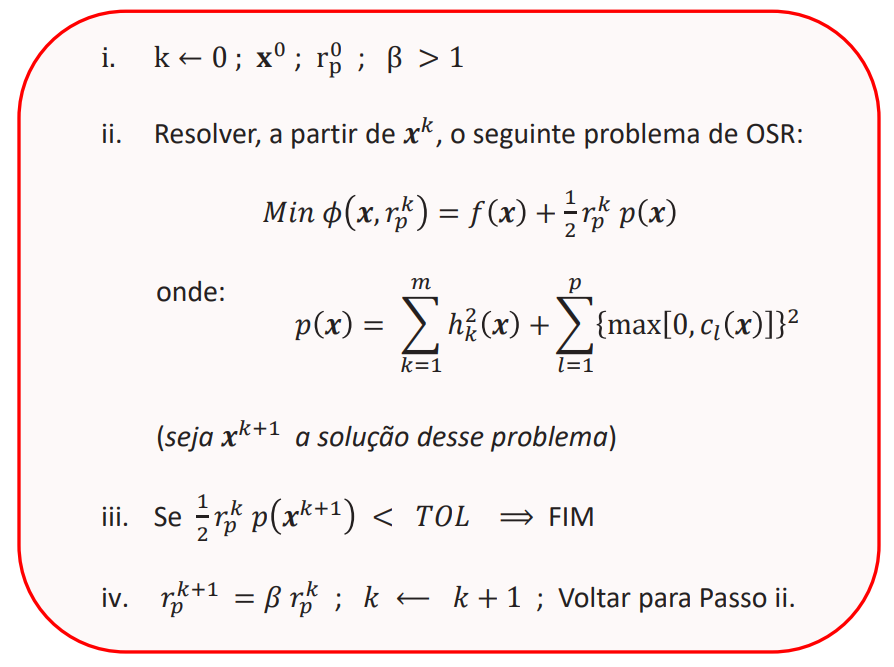
\includegraphics[width=.6\textwidth]{algoritmoPenalidade.PNG}
      \caption{Principais passos do m\'etodo da penalidade (\cite{ppt})}
      \label{fig:algoritmoPenalidade}
\end{figure}

\subsection{M\'etodo da Barreira}

No m\'etodo da barreira (ou m\'etodo interior), a converg\^encia se d\'a do interior da regi\~ao das solu\c c\~oes vi\'aveis para o contorno dela. Essa caracter\'istica torna a solu\c c\~ao em cada itera\c c\~ao do processo uma solu\c c\~ao vi\'avel, o que \'e interessante. O m\'etodo usa a denomina\c c\~ao barreira porque a fun\c c\~ao de barreira se torna infinita no contorno da regi\~ao vi\'avel.

\begin{equation} \label{eqBarr}
      \phi (\vec{x}, r_p) = f(\vec{x}) + r_b \sum_{k=1}^{m} h_k^2(\vec{x}) + r_b \sum_{l=1}^{p} - \frac{1}{c_l(\vec{x})}
\end{equation}

Como, no caso da barreira, a solu\c c\~ao converge pela regi\~ao vi\'avel, $c_l \leq 0$ e, portanto, existe um sinal negativo na eq. \ref{eqBarr} para tornar a pseudo-fun\c c\~ao objetivo $\phi$ postiva e, consequentemente, permitir sua minimiza\c c\~ao, caso contr\'ario esta iria para $-\infty$, j\'a que $c_l$ tende a se aproximar de zero \`a medida que as itera\c c\~oes avan\c cam.

O passo a passo do m\'etodo da barreira \'e descrito na figura \ref{fig:algoritmoBarreira}

\begin{figure}[H]
      \centering
      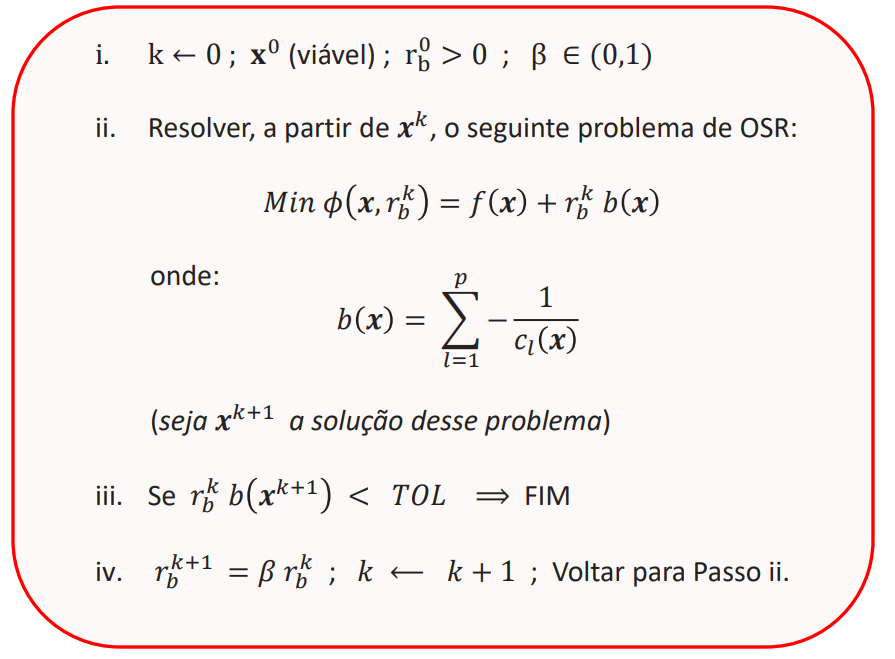
\includegraphics[width=.6\textwidth]{algoritmoBarreira.PNG}
      \caption{Principais passos do m\'etodo da barreira (\cite{ppt})}
      \label{fig:algoritmoBarreira}
\end{figure}

\section{Metodologia}

O fluxo de trabalho para solu\c c\~ao do problema de OCR est\'a descrito na figura \ref{fig:workflow} a seguir \'e v\'alido tanto para o m\'etodo de penalidade quanto para o m\'etodo de barreira.

O primeiro passo \'e a inicializa\c c\~ao das fun\c c\~oes $f$, suas restri\c c\~oes $c_l$, que no caso dos problemas propostos s\~ao apenas de desigualdade, al\'em da escolha do ponto inicial $x^0$. Em seguida procede-se a escolha dos par\^ametros dos algoritmos de OSR e OCR: Toler\^ancias para verifica\c c\~ao da converg\^encia, $d\alpha$, $\beta$ e $r_p$ (ou $r_b$).

Em seguida cria-se um looping de $m=1...6$ para varrer todos os m\'etodos de OSR: Univariante, Powell, Steepest-Descent, Fletcher-Reeves, Newton-Raphson e BFGS.

 Para cada um desses m\'etodos cria-se o termo de penaliza\c c\~ao $p(\vec{x})$ ou $b(\vec{x})$ e a pseudo-fun\c c\~ao objetivo $\phi(\vec{x}, r)$, al\'em das fun\c c\~oes $\vec{\nabla} \phi(\vec{x}, r)$ e $\vec{H}(\phi(\vec{x}, r))$. Esses manipuladores de fun\c c\~ao s\~ao passados para o script OSR juntamente com o ponto $x^0$ para solu\c c\~ao do problema de otimiza\c c\~ao sem restri\c c\~ao da fun\c c\~ao $\phi$.

 Ap\'os a solu\c c\~ao de $x^k$ pelo m\'etodo de OSR, plota-se as curvas de n\'ivel de $\phi$ e todos os pontos de solu\c c\~ao $x^0$, $x^1$, .... $x^(k-1)$, $x^k$ at\'e o passo atual, para evidenciar graficamente a trajet\'oria da solu\c c\~ao.

 Por fim, avalia-se a convergencia do problema de OCR e caso n\~ao haja converg\^encia, proceder-se-\'a novo c\'alculo de $x^(k+1)$ a partir de $x^k$, para isso atualiza-se o valor de $r_p$ (ou $r_b$) e procede-se novo c\'alculo de OSR a partir do novo $x^k$. O passo a passo \'e repetido par todos os m\'etodos de busca direcional de OSR.

\begin{figure}[H]
      \centering
      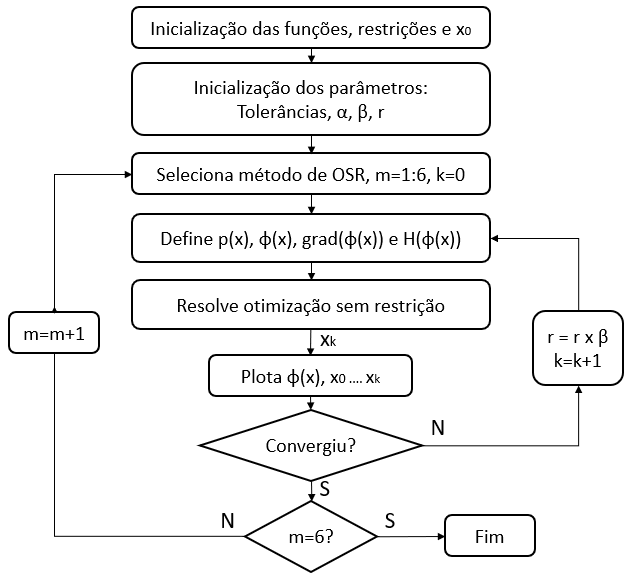
\includegraphics[width=.7\textwidth]{workflow.PNG}
      \caption{Passo a passo para solu\c c\~ao do problema de OCR}
      \label{fig:workflow}
\end{figure}

Os principais trechos dos scripts \textit{Matlab} utilizados ser\~ao listados na se\c c\~ao Anexos.

\section{Resultados}

Visando a converg\^encia de todos os m\'etodos, foram testados alguns valores dos par\^ametros dos algoritmos. A melhor combina\c c\~ao dos par\^ametros, para as fun\c c\~oes dos problemas 1 e 2 em termos de converg\~encia dos algoritmos est\'a listada na tabela \ref{table:params}.

O processo de busca linear implementado para solu\c c\~ao do problema de OSR possui inefici\^encias e imperfei\c c\~oes, principalmente no caso das fun\c c\~oes-objetivo serem mais complexas quando associadas aos termos de penalidade, conforme \'e o caso das pseudo-fun\c c\~os objetivo associadas aos casos de OCR. Este fato levou a dificuldades na converg\^encia dos algortimos, em geral.

Foram testados valores de toler\^ancias menores, na faixa de $10^{-6}$, e $d\alpha$ (passo da busca linear) maiores. Nesses casos, os algortimos at\'e convergiam, por\'em em temos muito longos, o que prejudicou a possibilidade de testes e execu\c c\~ao do trabalho. Dessa forma, o programa implementado para a solu\c c\~ao dos problemas de OCR utilizou os valores da tabela \ref{table:params}.

Outro par\^ametro relevante foi n\'umero m\'aximo de itera\c c\~oes do algoritmo de OSR, para evitar que o algoritmo ficasse indefinidamente na busca pelo m\'inimo da fun\c c\~ao $\phi$, o que aconteceu para alguns valores de $r$, principalmente no problema 2 (barreira)

\small
$$
\text{Par\^ametros:} \begin{cases}
      \text{$d\alpha$:  tamanho do passo do algoritmo do passo constante}\\
      \text{TOL(BL):    toler\^ancia associada ao algoritmo da Busca Linear no problema de OSR}\\
      \text{TOL(OCR):   toler\^ancia utilizada para verificar a converg\^encia dos algortimos de OCR}\\
      \text{TOL(SA):    toler\^ancia associada ao algoritmo da Se\c c\~ao \'Aurea no problema de OSR}\\
      \text{$\beta$:    multiplicados do termo de penaliza\c c\~ao $r$ da pseudo-fun\c c\~ao objetivo do algoritmo de OCR}\\
      \text{iter\_max:  m\'aximo n\'umero de itera\c c\~oes do algoritmo de OSR}
\end{cases}
$$
\normalsize

\begin{table}[H]
      \small
      \centering
      \caption{Melhores par\^ametros para converg\^encia dos algoritmos}
      \begin{tabular}{c|c|c|c|c|c|c|c}
            Problema & M\'etodo & Algoritmo & $d\alpha$ & TOL(BL) & TOL(OCR) & TOL(SA) & $\beta$\\
            \hline
            \multirow{6}{*}{01} & \multirow{6}{*}{Penalidade} & Univariante       & 0.002 & $10^{-4}$ & $10^{-4}$ & $10^{-6}$ & 5   \\
                                                            & & Powell            & 0.002 & $10^{-4}$ & $10^{-4}$ & $10^{-5}$ & 10  \\
                                                            & & Steepest Descent  & 0.002 & $10^{-4}$ & $10^{-4}$ & $10^{-9}$ & 5   \\
                                                            & & Flecher-Reeves    & 0.001 & $10^{-4}$ & $10^{-4}$ & $10^{-7}$ & 5   \\
                                                            & & Newton-Raphson    & 0.05  & $10^{-4}$ & $10^{-4}$ & $10^{-7}$ & 20  \\
                                                            & & BFGS              & 0.04  & $10^{-5}$ & $10^{-5}$ & $10^{-8}$ & 10  \\
            \hline
            \multirow{6}{*}{01} & \multirow{6}{*}{Barreira} & Univariante         & 0.0002 & $10^{-4}$ & $10^{-4}$ & $10^{-8}$ & 0.05 \\
                                                            & & Powell            & 0.0002 & $10^{-4}$ & $10^{-4}$ & $10^{-5}$ & 0.2  \\
                                                            & & Steepest Descent  & 0.0002 & $10^{-4}$ & $10^{-4}$ & $10^{-7}$ & 0.05 \\
                                                            & & Flecher-Reeves    & 0.0002 & $10^{-4}$ & $10^{-4}$ & $10^{-7}$ & 0.05 \\
                                                            & & Newton-Raphson    & 0.002  & $10^{-6}$ & $10^{-6}$ & $10^{-7}$ & 0.05 \\
                                                            & & BFGS              & 0.0002 & $10^{-4}$ & $10^{-4}$ & $10^{-5}$ & 0.05 \\
            \hline
            \multirow{6}{*}{02} & \multirow{6}{*}{Penalidade} & Univariante       & 0.005  & $10^{-6}$ & $10^{-6}$ & $10^{-7}$ & 10 \\
                                                            & & Powell            & 0.005  & $10^{-6}$ & $10^{-6}$ & $10^{-5}$ & 50 \\
                                                            & & Steepest Descent  & 0.0001 & $10^{-3}$ & $10^{-4}$ & $10^{-7}$ & 10 \\
                                                            & & Flecher-Reeves    & 0.0001 & $10^{-3}$ & $10^{-4}$ & $10^{-7}$ & 10 \\
                                                            & & Newton-Raphson    & 0.0002 & $10^{-5}$ & $10^{-6}$ & $10^{-7}$ & 10 \\
                                                            & & BFGS              & 0.0002 & $10^{-3}$ & $10^{-4}$ & $10^{-7}$ & 10 \\
            \hline
            \multirow{6}{*}{02} & \multirow{6}{*}{Barreira} & Univariante         & 0.0001  & $10^{-4}$ & $10^{-4}$ & $10^{-9}$  & 0.12   \\
                                                            & & Powell            & 0.0001  & $10^{-4}$ & $10^{-4}$ & $10^{-10}$ & 0.09   \\
                                                            & & Steepest Descent  & 0.00002 & $10^{-4}$ & $10^{-4}$ & $10^{-9}$  & 0.005  \\
                                                            & & Flecher-Reeves    & 0.00002 & $10^{-4}$ & $10^{-4}$ & $10^{-7}$  & 0.008  \\
                                                            & & Newton-Raphson    & 0.001   & $10^{-6}$ & $10^{-6}$ & $10^{-6}$  & 0.01   \\
                                                            & & BFGS              & 0.0002  & $10^{-5}$ & $10^{-4}$ & $10^{-8}$  & 0.0006 \\
            \hline
      \end{tabular}
      \label{table:params}
\end{table}


A tabela \ref{table:results} abaixo ilustra os resultados encontrados para a implementa\c c\~ao dos m\'etodos de penalidade e barreira para as fun\c c\~oes e restri\c c\~oes dos problemas 01 e 02. Al\'em dos pontos de m\'inimo encontrados, a tabela apresenta tamb\'em o n\'umero de passos para a converg\^encia e o tempo de execu\c c\~ao. Estes dois \'ultimos representam quantas vezes foi chamado o script de solu\c c\~ao do problema de OSR e quanto tempo computacional foi consumido no total de itera\c c\~oes, respectivamente.

\begin{table}[H]
      \small
      \centering
      \caption{Resultados}
      \begin{tabular}{c|c|c|c|c|c|c}
            Problema & M\'etodo, $x^0$  & Algoritmo & $x^{min}$ & passos & $\Delta t$(ms) \\
            \hline
            \multirow{6}{*}{01} & \multirow{6}{*}{Penalidade, $x^0=\{3,2\}$} & Univariante       & $\{0.9446,0.8921\}$ & 8 & 55.3  \\
                                                            & & Powell            & $\{0.9456,0.8941\}$ & 6 & 198.4 \\
                                                            & & Steepest Descent  & $\{0.9456,0.8941\}$ & 8 & 20.8  \\
                                                            & & Flecher-Reeves    & $\{0.9456,0.8941\}$ & 8 & 5.9   \\
                                                            & & Newton-Raphson    & $\{0.9456,0.8941\}$ & 5 & 3.9   \\
                                                            & & BFGS              & $\{0.9456,0.8941\}$ & 7 & 2.4   \\
            \hline
            \multirow{6}{*}{01} & \multirow{6}{*}{Barreira, $x^0=\{0,1\}$} & Univariante         & $\{0.9467,0.8969\}$ & 6  & 78.0   \\
                                                            & & Powell            & $\{0.9453,0.8944\}$ & 11 & 8615.5 \\
                                                            & & Steepest Descent  & $\{0.9456,0.8948\}$ & 6  & 797.9  \\
                                                            & & Flecher-Reeves    & $\{0.9454,0.8944\}$ & 6  & 297.1  \\
                                                            & & Newton-Raphson    & $\{0.9456,0.8941\}$ & 10 & 124.0  \\
                                                            & & BFGS              & $\{0.9454,0.8944\}$ & 6  & 239.1  \\
            \hline
            \multirow{6}{*}{02} & \multirow{6}{*}{Penalidade, $x^0=\{1,15\}$} & Univariante       & $\{1.8784,20.2363\}$ & 15 & 144.3   \\
                                                            & & Powell            & $\{1.8783,20.2365\}$ & 8  & 247.3   \\
                                                            & & Steepest Descent  & $\{1.8784,20.2357\}$ & 14 & 5302.9  \\
                                                            & & Flecher-Reeves    & $\{1.8783,20.2350\}$ & 12 & 1920.4  \\
                                                            & & Newton-Raphson    & $\{1.8783,20.2365\}$ & 15 & 528.7   \\
                                                            & & BFGS              & $\{1.8783,20.2363\}$ & 13 & 6433.7  \\
            \hline
            \multirow{6}{*}{02} & \multirow{6}{*}{Barreira, $x^0=\{4,25\}$} & Univariante         & $\{1.8785,20.2389\}$ & 15 & 13461.8 \\
                                                            & & Powell            & $\{1.8785,20.2396\}$ & 13 & 11053.0 \\
                                                            & & Steepest Descent  & $\{1.8793,20.8871\}$ & 5  & 9248.0  \\
                                                            & & Flecher-Reeves    & $\{1.8855,20.3466\}$ & 5  & 3708.0  \\
                                                            & & Newton-Raphson    & $\{1.8784,20.2367\}$ & 8  & 225.5   \\
                                                            & & BFGS              & $\{1.8971,20.5055\}$ & 3  & 1675.9  \\
            \hline
      \end{tabular}
      \label{table:results}
\end{table}

\newpage

Conforme citado anteriormente, a utliza\c c\~ao de m\'etodos indiretos em OCR consiste na incorpora\c c\~ao das restri\c c\~oes na fun\c c\~ao objetivo a ser minimizada, sendo os termos associados \`as restri\c c\~oes penalizados gradualmente.

Nas figuras a seguir, para cada passo dos algoritmos de penalidade ou barreira, ilustra-se as curvas de n\'ivel da pseudo-fun\c c\~ao objetivo $\phi(x_1, x_2)$, onde se pode evidenciar a forma que esta vai tomando a cada passo do m\'etodo, a partir da incorpora\c c\~ao e penaliza\c c\~ao dos termos de restri\c c\~ao.

Sobrepostos \`as curvas de n\'ivel de $\phi(x_1, x_2)$, para cada passo $k=1....n$ ilustra-se o conjunto de pontos $\{x^0, x^1, ... , x^k\}$ (solu\c c\~oes do problema de OSR) at\'e o passo atual.

%%%%%%%%%%%%%%%%%%%%%%%%%%%
% PROBLEMA 01
%%%%%%%%%%%%%%%%%%%%%%%%%%%

As figuras a seguir ilustram as curvas da solu\c c\~ao de OCR para a fun\c c\~ao a as restri\c c\~oes do problema 1

Na figura \ref{fig:fig01} podemos ver a regi\~ao vi\'avel (acima da curva vermelha) e a converg\^encia do algoritmo pelo algortimo de Powell de OSR pelo m\'etodo da penalidade, assim como a deforma\c c\~ao de $\phi(x_1,x_2)$ a partir do ponto $x^0=\{3,2\}$. Nota-se tamb\'em a converg\^encia do algoritmo pela regi\~ao n\~ao vi\'avel (abaixo da curva vermelha).

\begin{figure}[H]
      \centering
      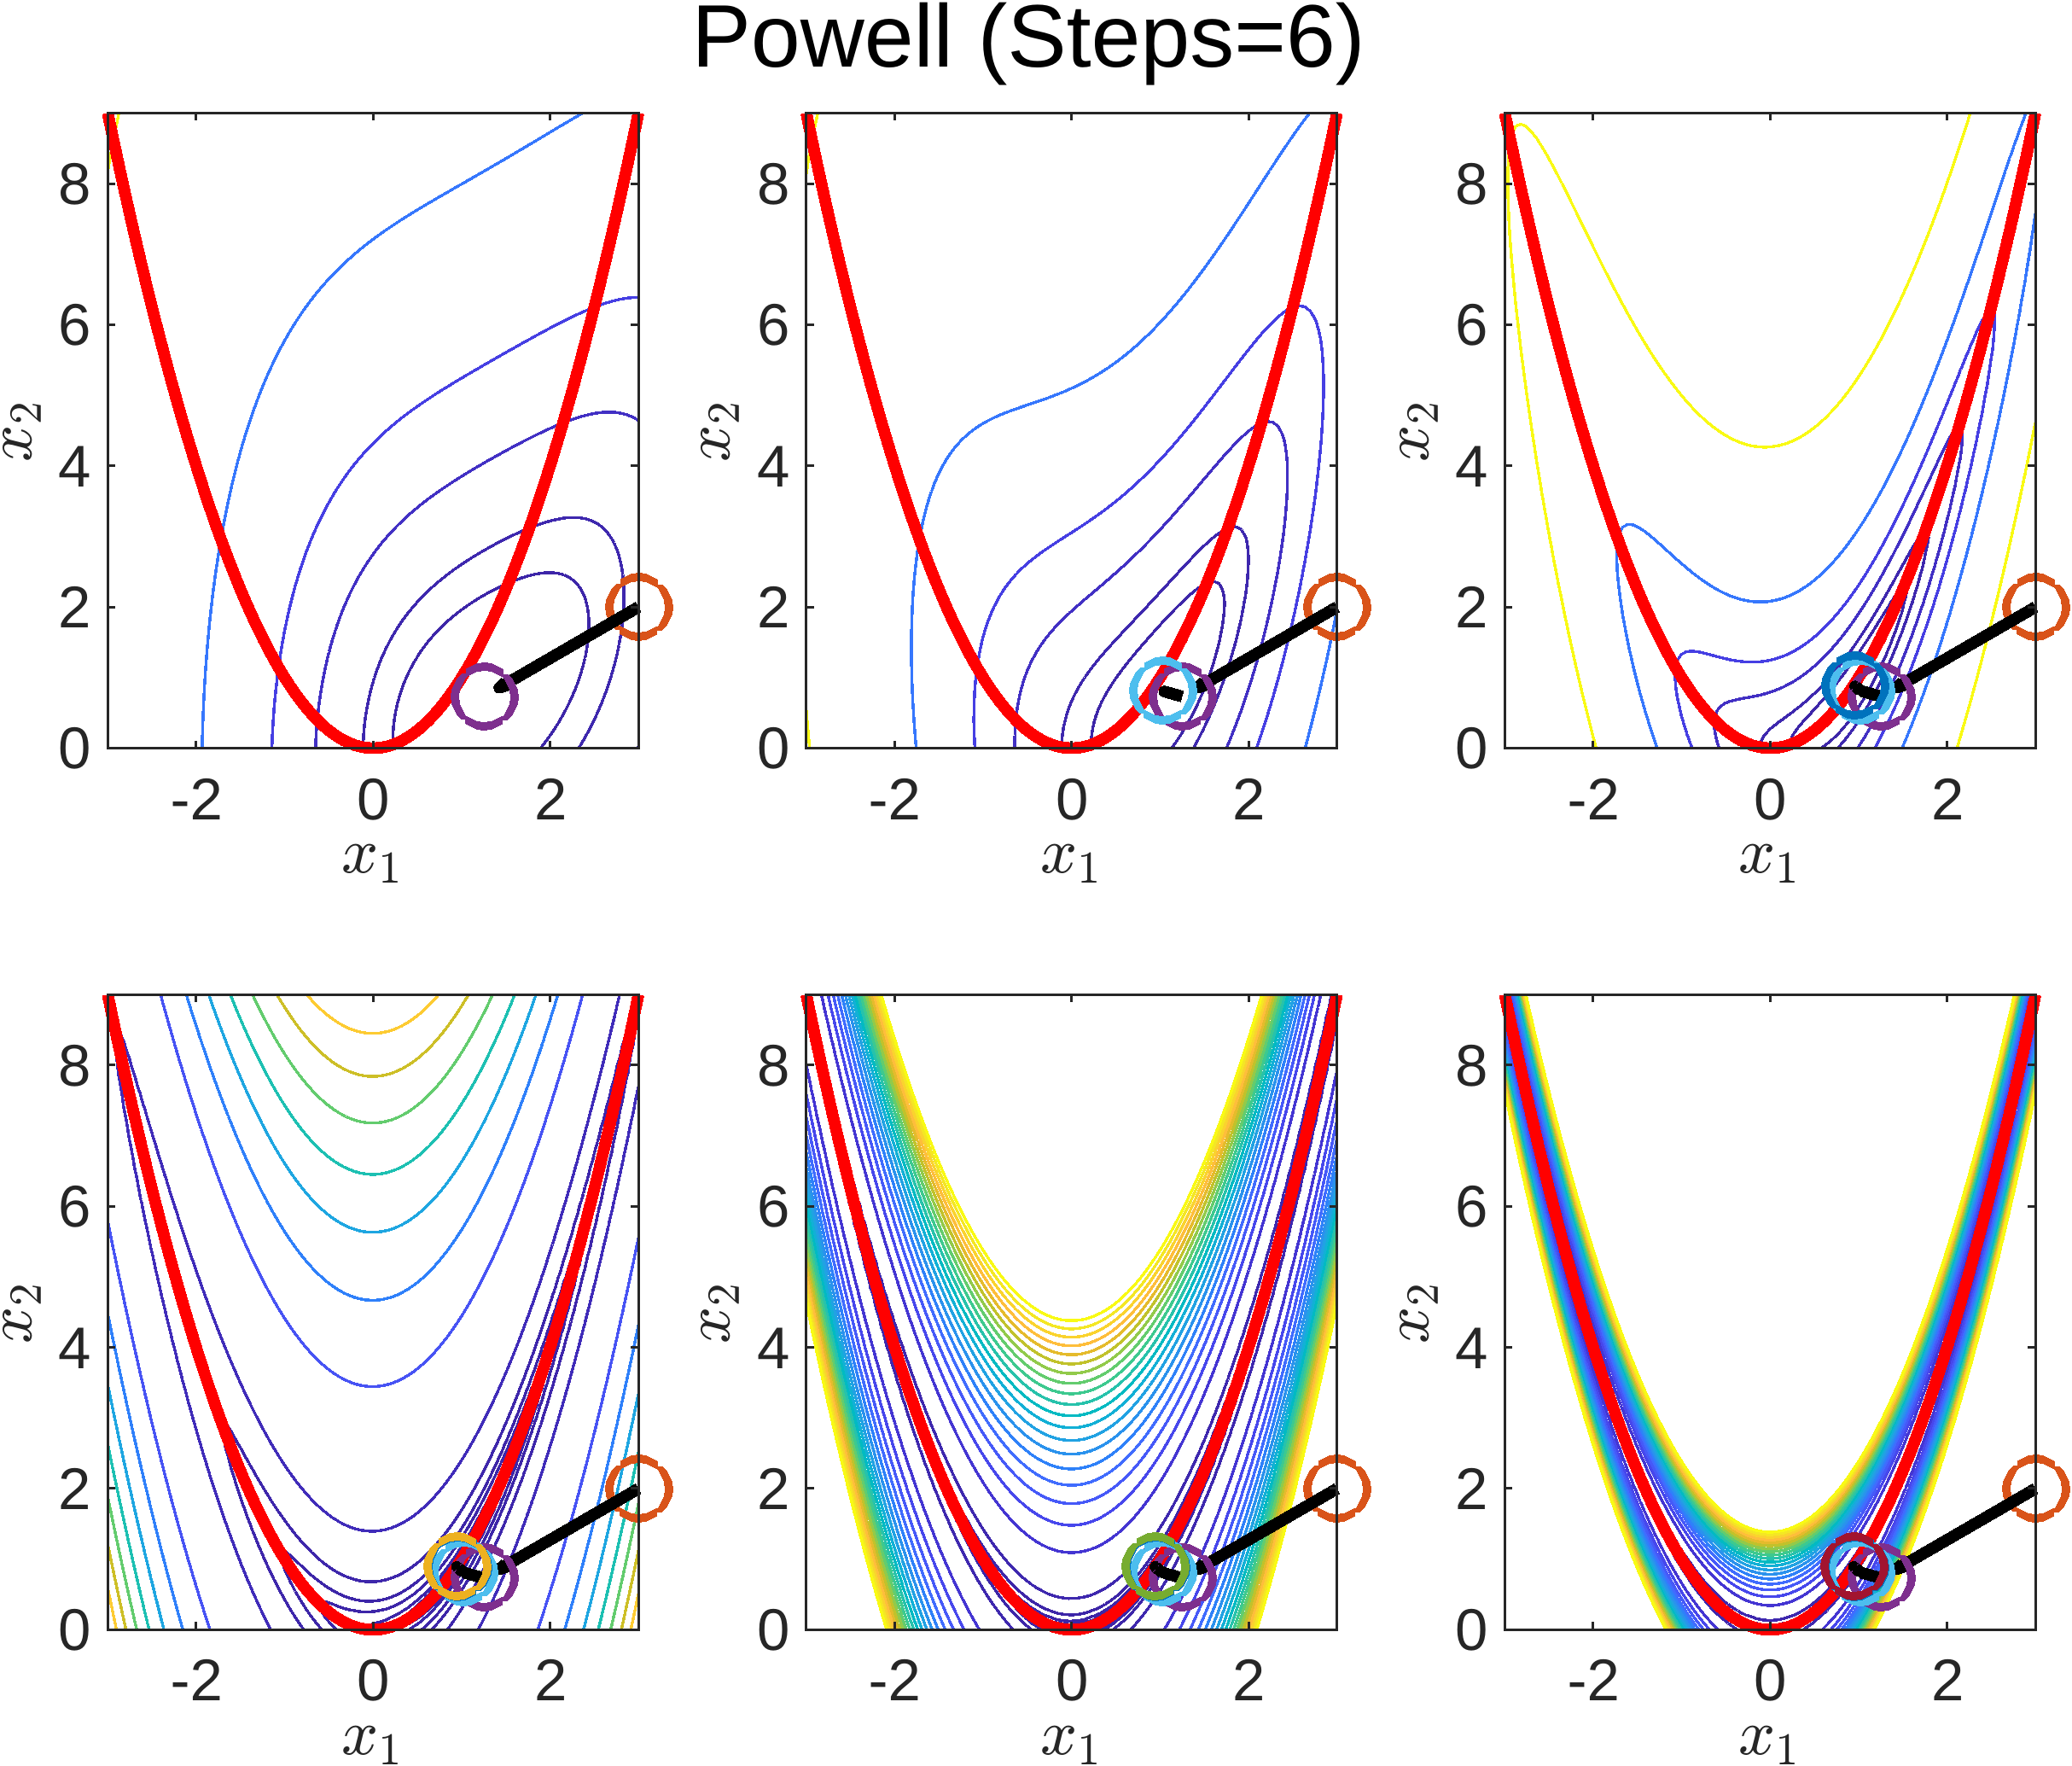
\includegraphics[width=0.75\textwidth]{fig01_P01_PEN_X1_POW.png}
      \caption{OCR do problema 01 pelo m\'etodo da penalidade, a partir do ponto $x^0=\{3,2\}$ - Algoritmo de Powell}
      \label{fig:fig01}
\end{figure}

Para avaliar a robustez dos algoritmos, selecionamos um novo ponto $x^0=\{0,4\}$, desta vez dentro da regi\~ao vi\'avel, uma vez que, diferente do m\'etodo de barreira, n\~ao \'e uma exig\^encia do algortimo que o ponto inicial seja um ponto vi\'avel. Nota-se que logo no primeiro passo, a solu\c c\~ao de OSR de $\phi$ converge para m\'inimo da fun\c c\~ao $f$, j\'a que, como $x^0$ \'e vi\'avel, esse n\~ao \'e computado em $\phi$ e esta fica igual a $f$. A partir da\'i, a sequencia do algoritmo segue pela regi\~ao n\~ao-vi\'avel. Na figura \ref{fig:fig02} ilustra-se tal caso pelo m\'etodo de Fletcher-Reeves.

\begin{figure}[H]
      \centering
      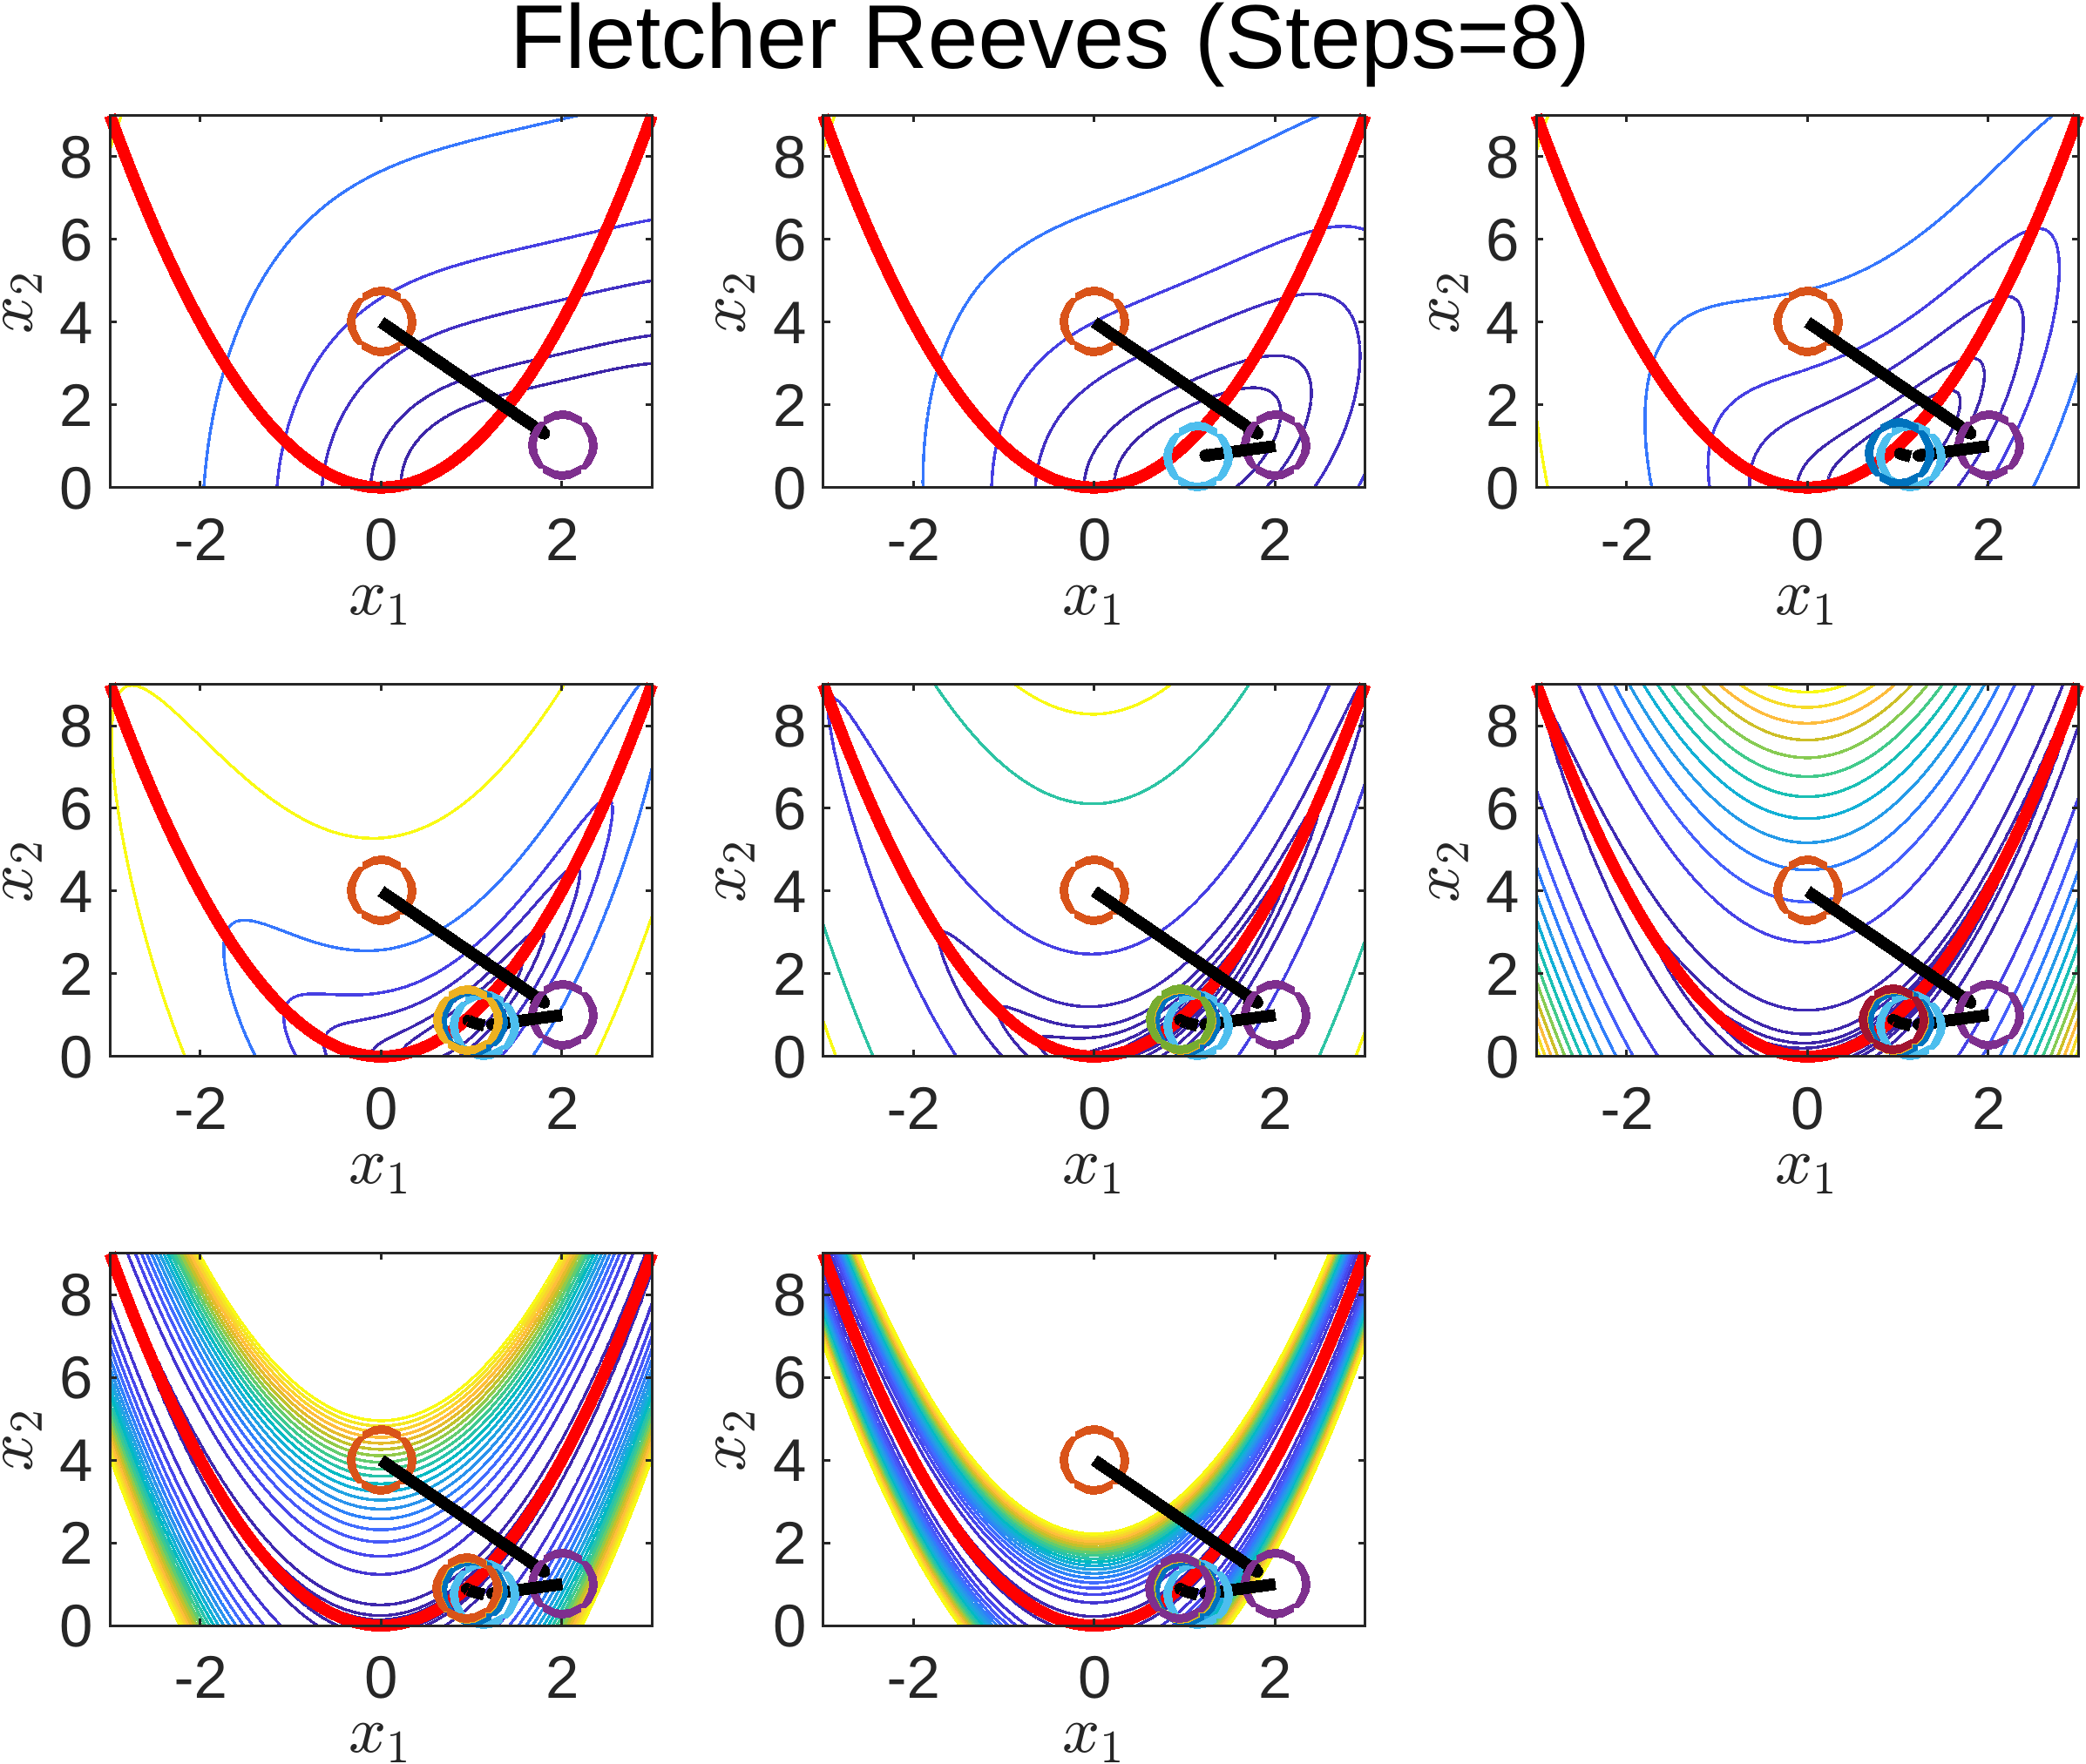
\includegraphics[width=0.75\textwidth]{fig02_P01_PEN_X2_FR.png}
      \caption{OCR do problema 01 pelo m\'etodo da penalidade, a partir do ponto $x^0=\{0,4\}$ - Algoritmo de Flecher-Reeves}
      \label{fig:fig02}
\end{figure}

Para o mesmo problema 01, a figura \ref{fig:fig03} a seguir ilustra a converg\^enia, pelo m\'etodo de OSR univariante, a partir do ponto $x^0=\{0,1\}$ e pelo m\'etodo de barreira.

Desta vez \'e poss\'ivel notar que a regi\~ao associada \`a restri\c c\~ao (curva vermelha) vai se tornando uma barreira nas curvas de n\'ivel de $\phi$. Aqui, \'e importante que a solu\c c\~ao, em qualquer passo $k$, $x^k$ permane\c ca vi\'avel, ou seja, $c_l(x^k)<=0$, caso contr\'ario, o ponto $x^k$ "romper\'a" a barreira e a fun\c c\~ao ir\'a convergir para um ponto na regi\~ao n\~ao vi\'avel.

\begin{figure}[H]
      \centering
      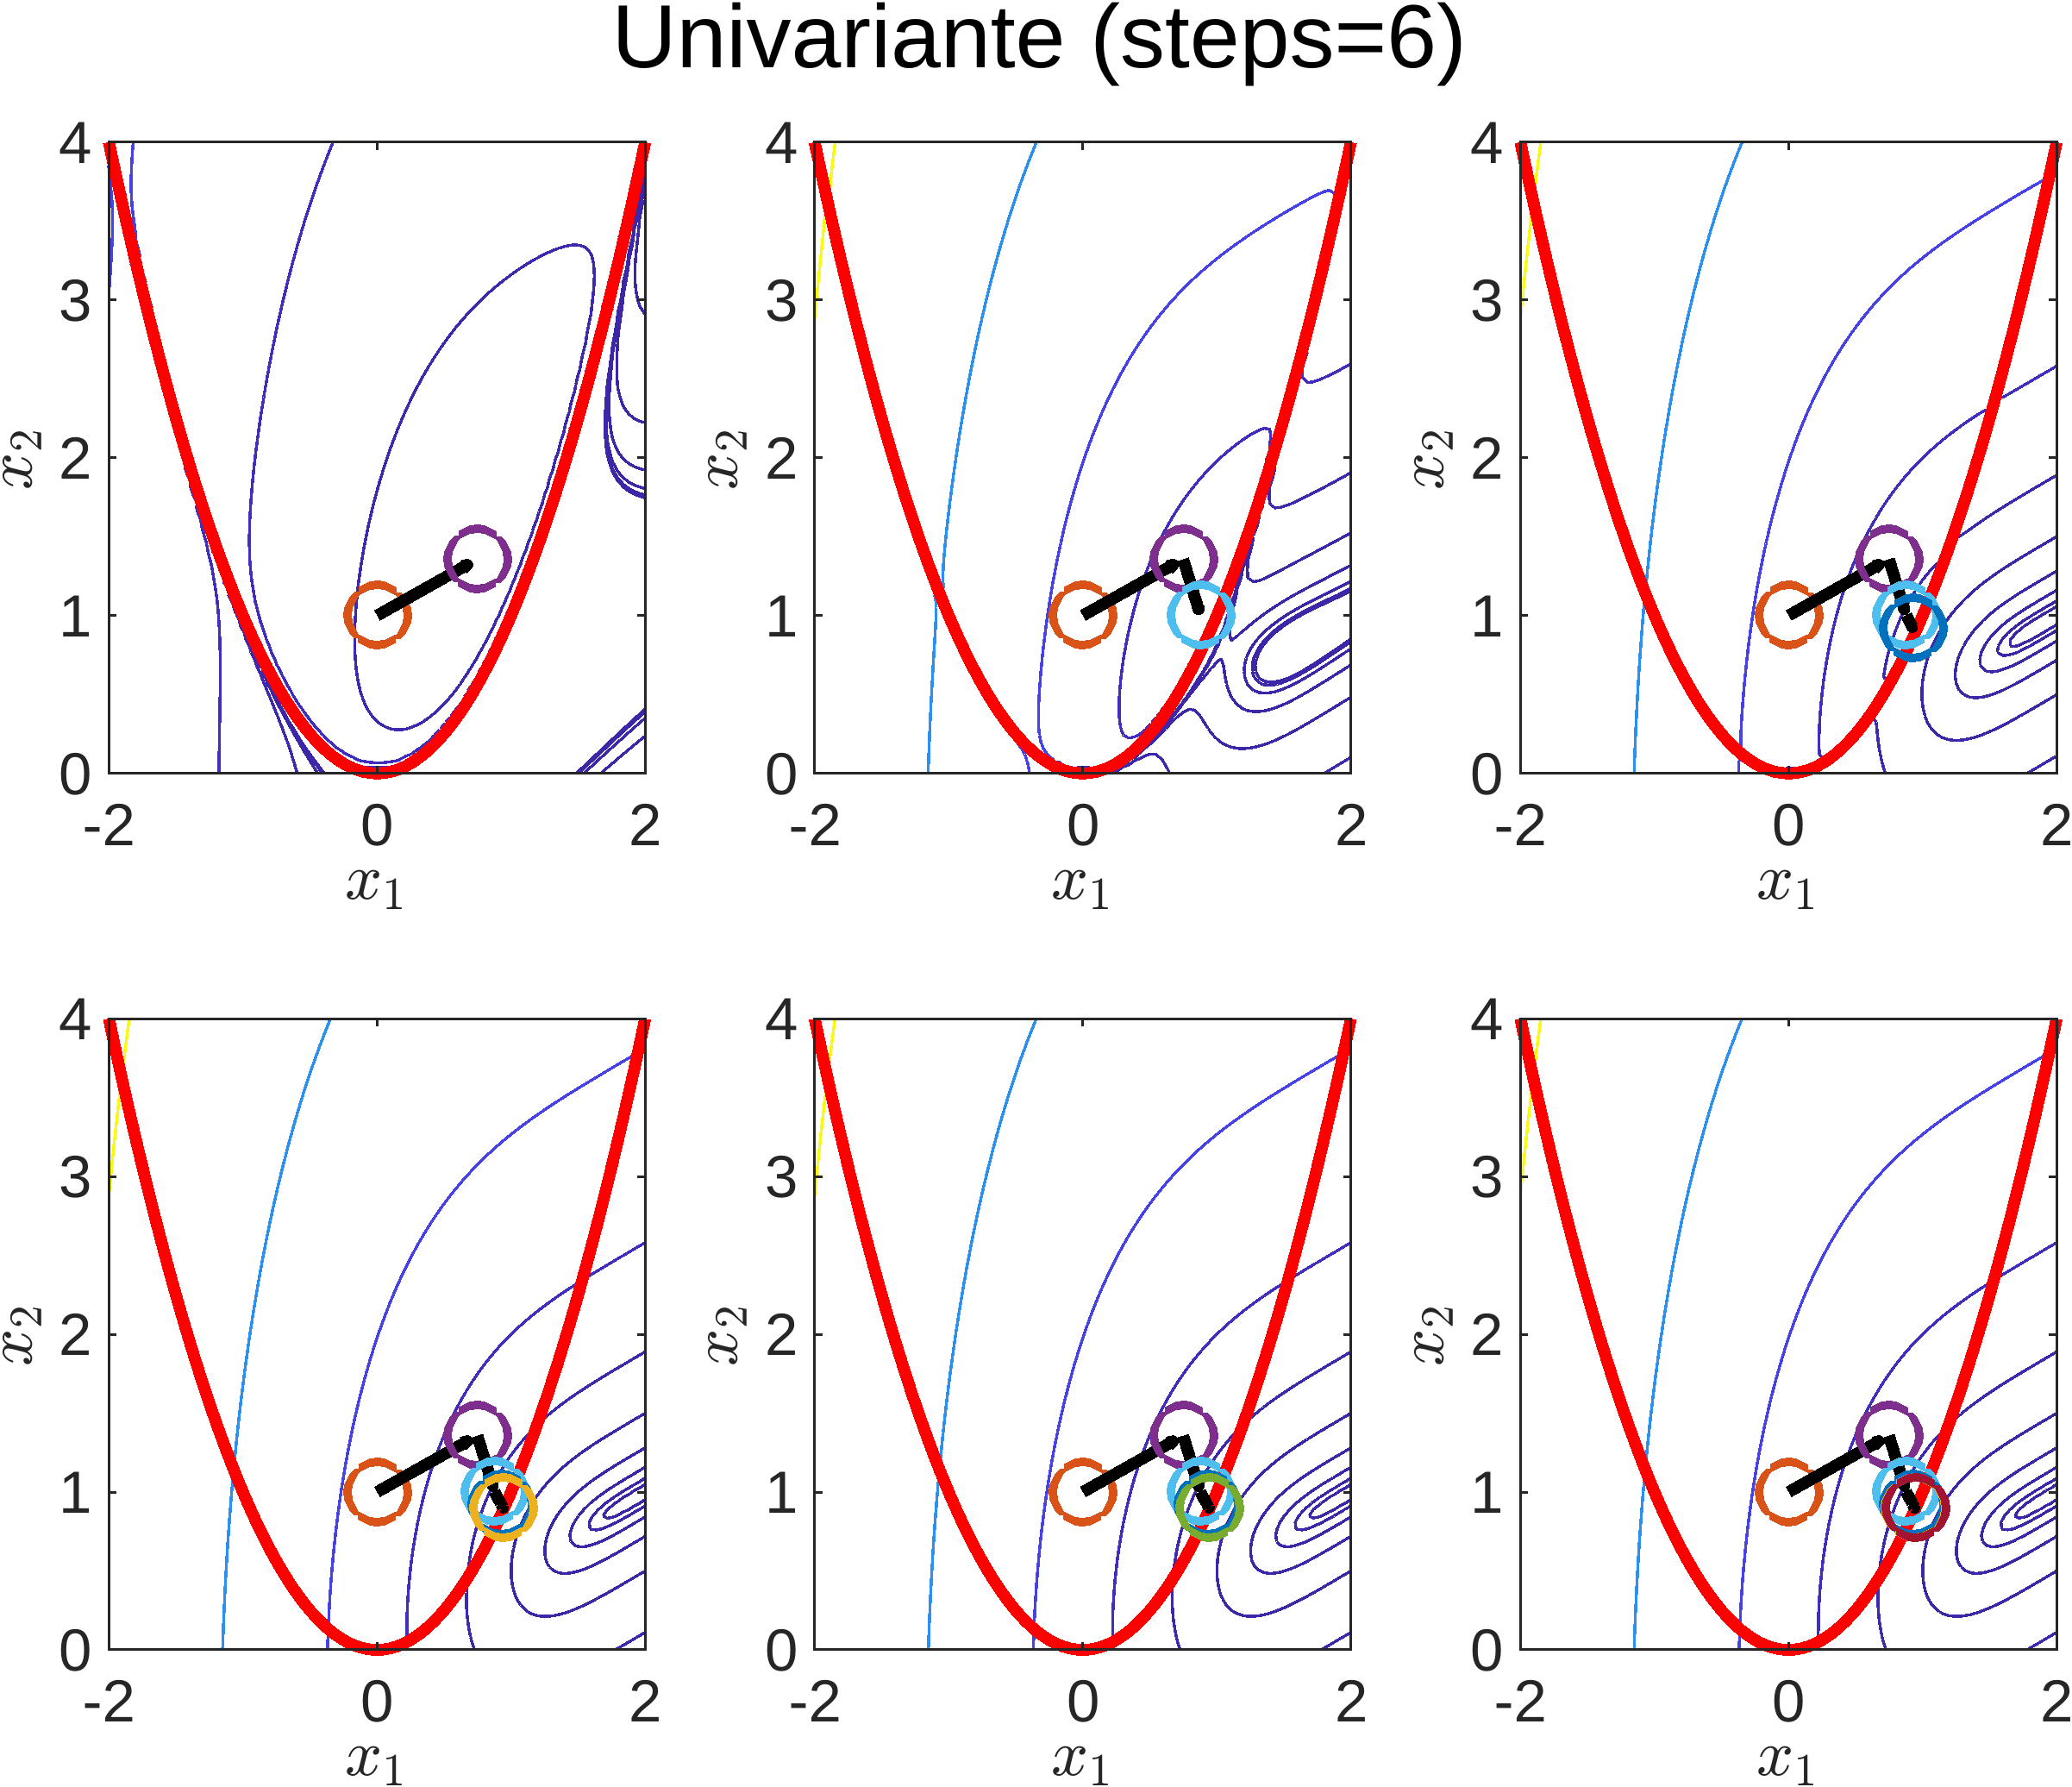
\includegraphics[width=0.75\textwidth]{fig03_P01_BAR_X1_UNI.png}
      \caption{OCR do problema 01 pelo m\'etodo da barreira, a partir do ponto $x^0=\{0,1\}$ - Algoritmo Univariante}
      \label{fig:fig03}
\end{figure}

Para melhor visualiza\c c\~ao da pseudo-fun\c c\~ao objetivo acima plotamos os gr\'aficos de curvas de n\'ivel e 3D da fun\c c\~ao da eq. \ref{eqPhi1B} nas figuras \ref{fig:wolf_contour} e \ref{fig:wolf_3d}, respectivamente, onde fica claro a regi\~ao associada \`a restri\c c\~ao como sendo uma "descontinuidade" de $\phi$ e porque o m\'etodo \'e chamado de m\'etodo de barreira.

\begin{equation} \label{eqPhi1B}
      \phi (x,y, r_b=1) = (x-2)^4 + (x-2y)^2 - \frac{rb}{x^2-y}
\end{equation}

\begin{figure}[H]
      \centering
      \begin{subfigure}{0.35\textwidth}
            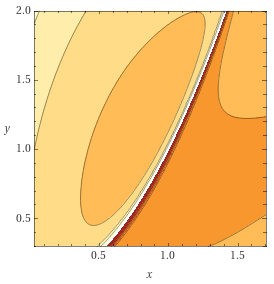
\includegraphics[width=\textwidth]{wolf_contour.PNG}
            \caption{contono de $\phi$}
            \label{fig:wolf_contour}
      \end{subfigure}
      \begin{subfigure}{0.45\textwidth}
            \centering
            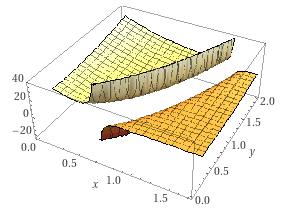
\includegraphics[width=\textwidth]{wolf_3d.PNG}
            \caption{3D plot de $\phi$}
            \label{fig:wolf_3d}
      \end{subfigure}
      \caption{Pseudo fun\c c\~ao objetivo do problema 01 (Barreira) com $rb=1$ (equa\c c\~ao \ref{eqPhi1B}), https://www.wolframalpha.com}
      \label{fig:wolf}
\end{figure}

Para avaliar a robustez do m\'etodo, selecionamos um novo ponto $x^0=\{2.5,10\}$, ainda vi\'avel. Na figura \ref{fig:fig04} ilustra-se tal caso pelo m\'etodo de Steepest-Descent.

\begin{figure}[H]
      \centering
      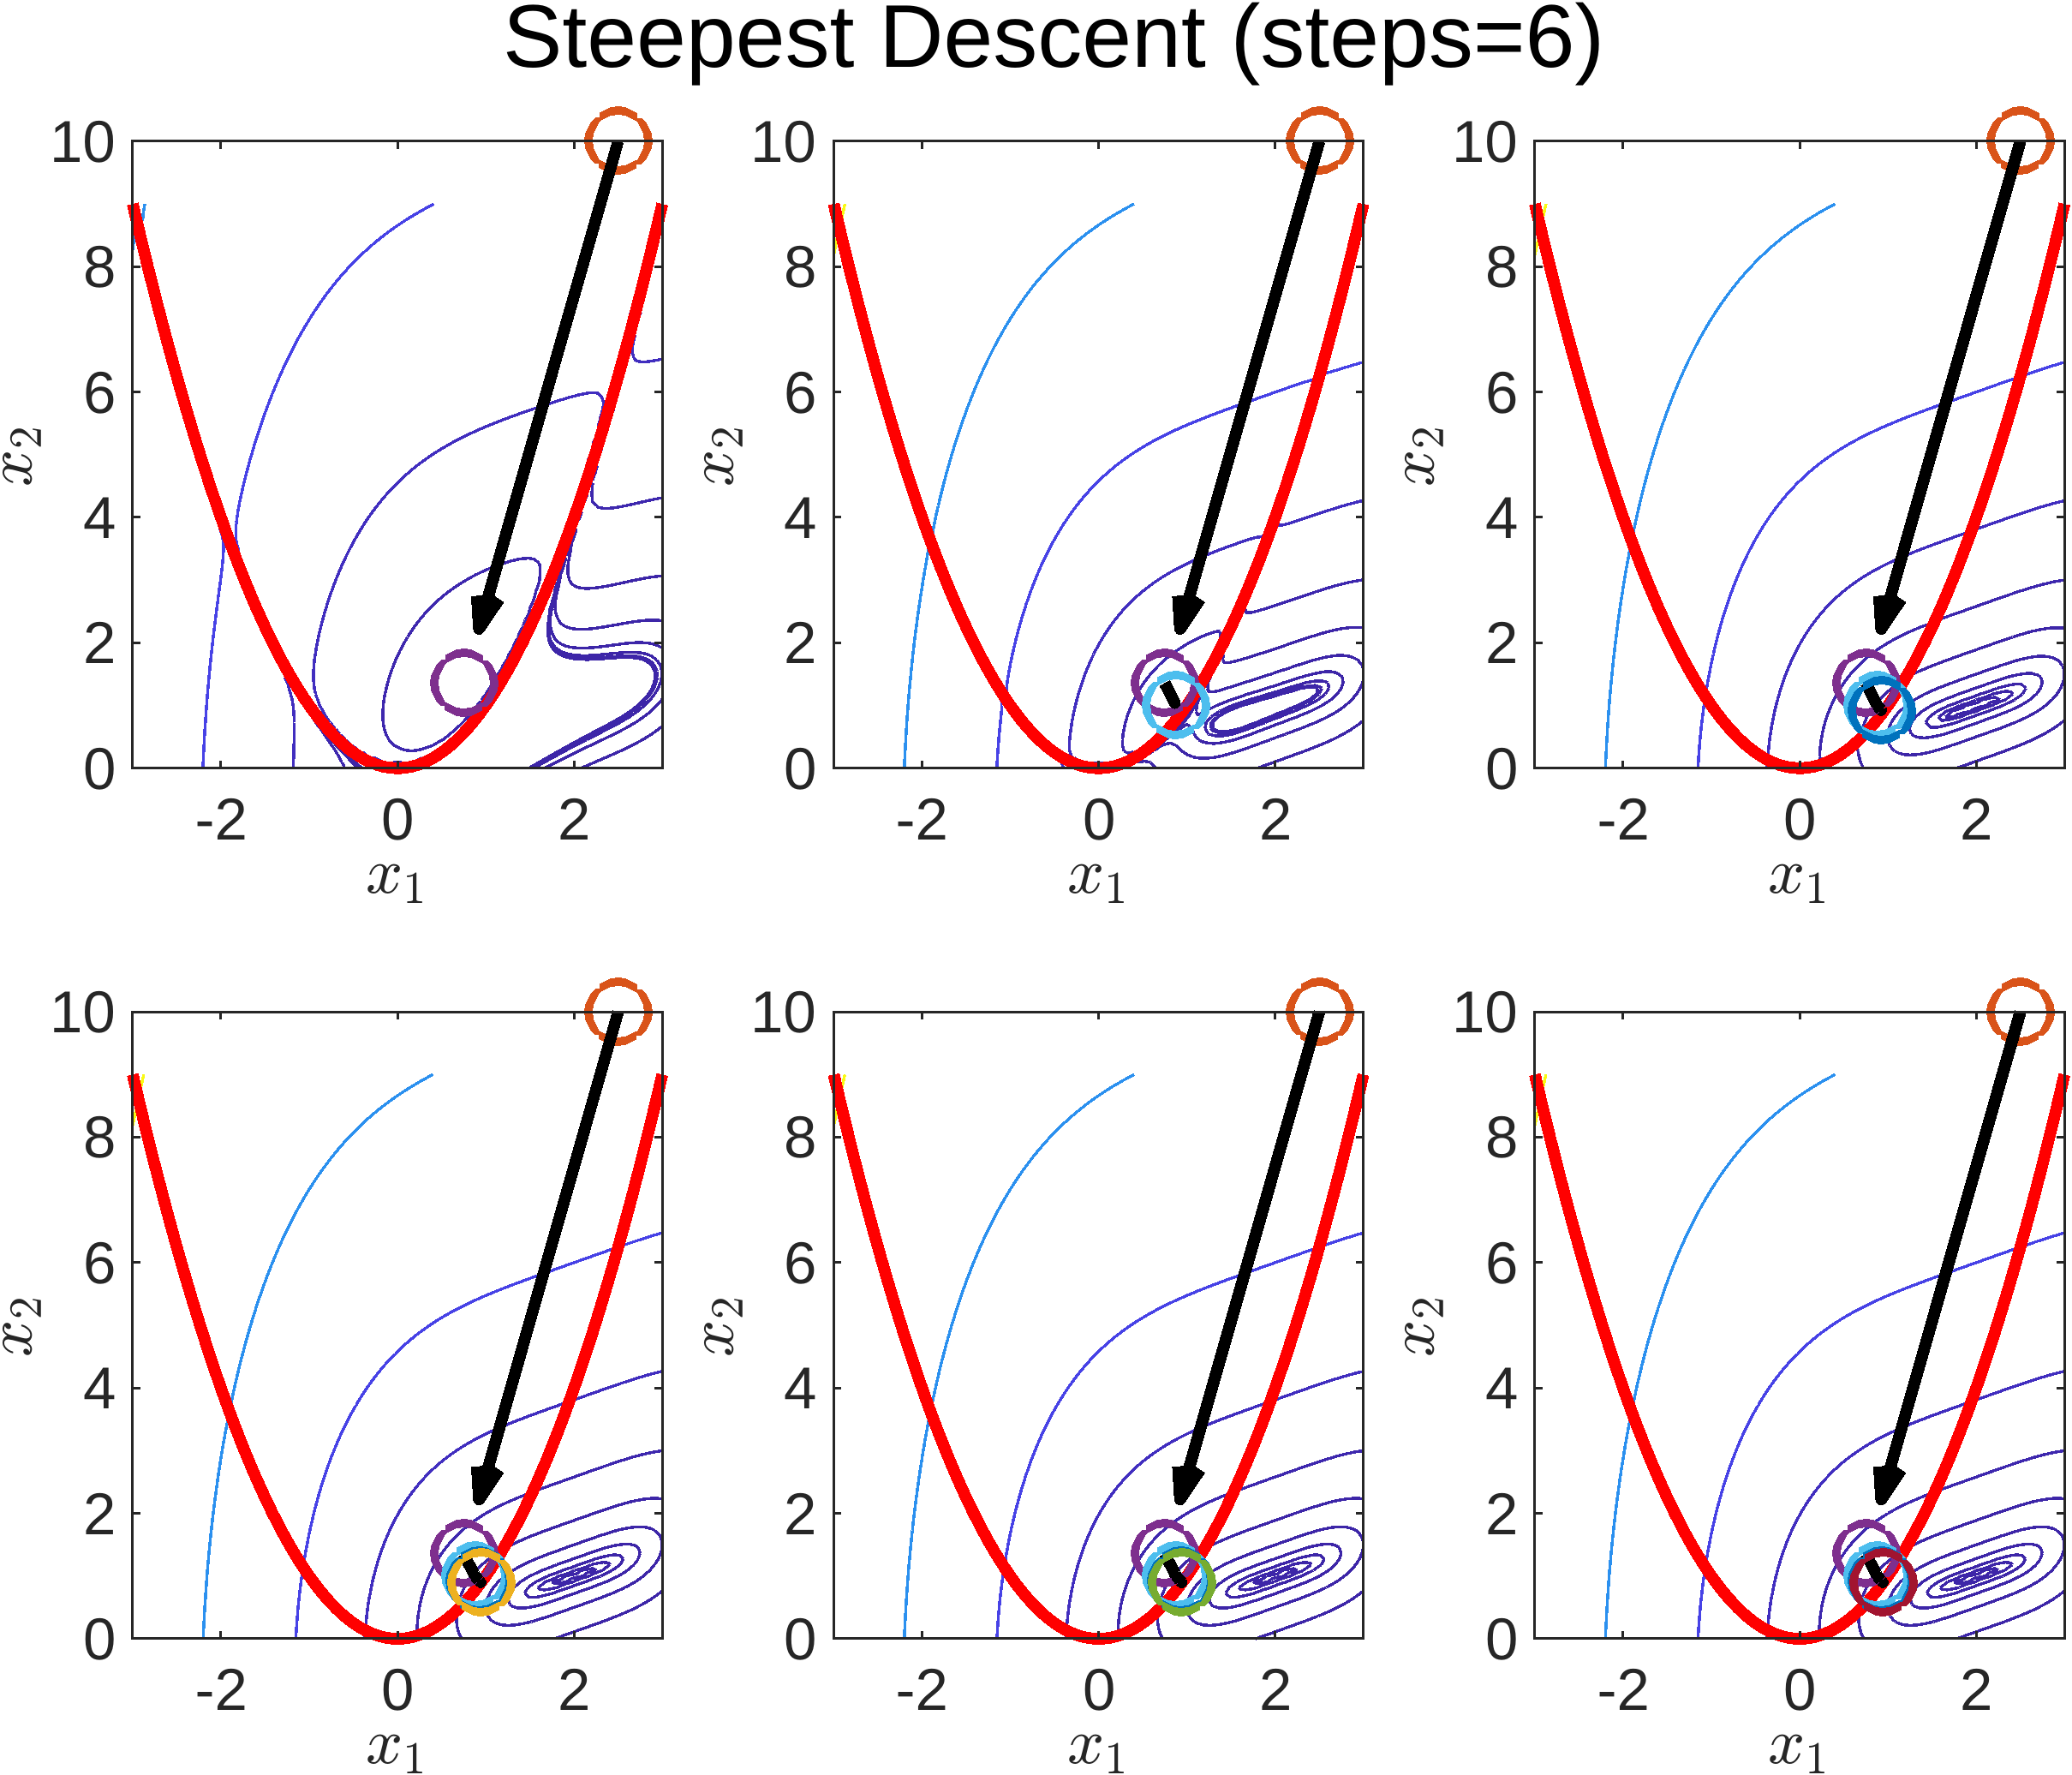
\includegraphics[width=0.75\textwidth]{fig04_P01_BAR_X2_SD.png}
      \caption{OCR do problema 01 pelo m\'etodo da barreira, a partir do ponto $x^0=\{2.5,10\}$ - Algoritmo Steepest Descent}
      \label{fig:fig04}
\end{figure}

%%%%%%%%%%%%%%%%%%%%%%%%%%%
% PROBLEMA 02
%%%%%%%%%%%%%%%%%%%%%%%%%%%

As figuras a seguir ilustram as curvas da solu\c c\~ao de OCR para a fun\c c\~ao a as restri\c c\~oes do problema 2

Nas figuras \ref{fig:fig05} e \ref{fig:fig06} a seguir ilustra-se as converg\^encias do algoritmo de OCR pelo m\'etodo de penalidade para dois pontos de partida distintos: $x^0=\{1,15\}$ e $x^0=\{3,3\}$, respecivamente. O primeiro utilizando, para OSR o m\'etodo de dire\c c\~oes de busca de Fletcher-Reeves e o segundo, Univariante.

Nota-se nesses dois gr\'aficos a maior complexidade da fun\c c\~ao e o consequente maior n\'umero de passos necess\'arios para converg\^encia.

\begin{figure}[H]
      \centering
      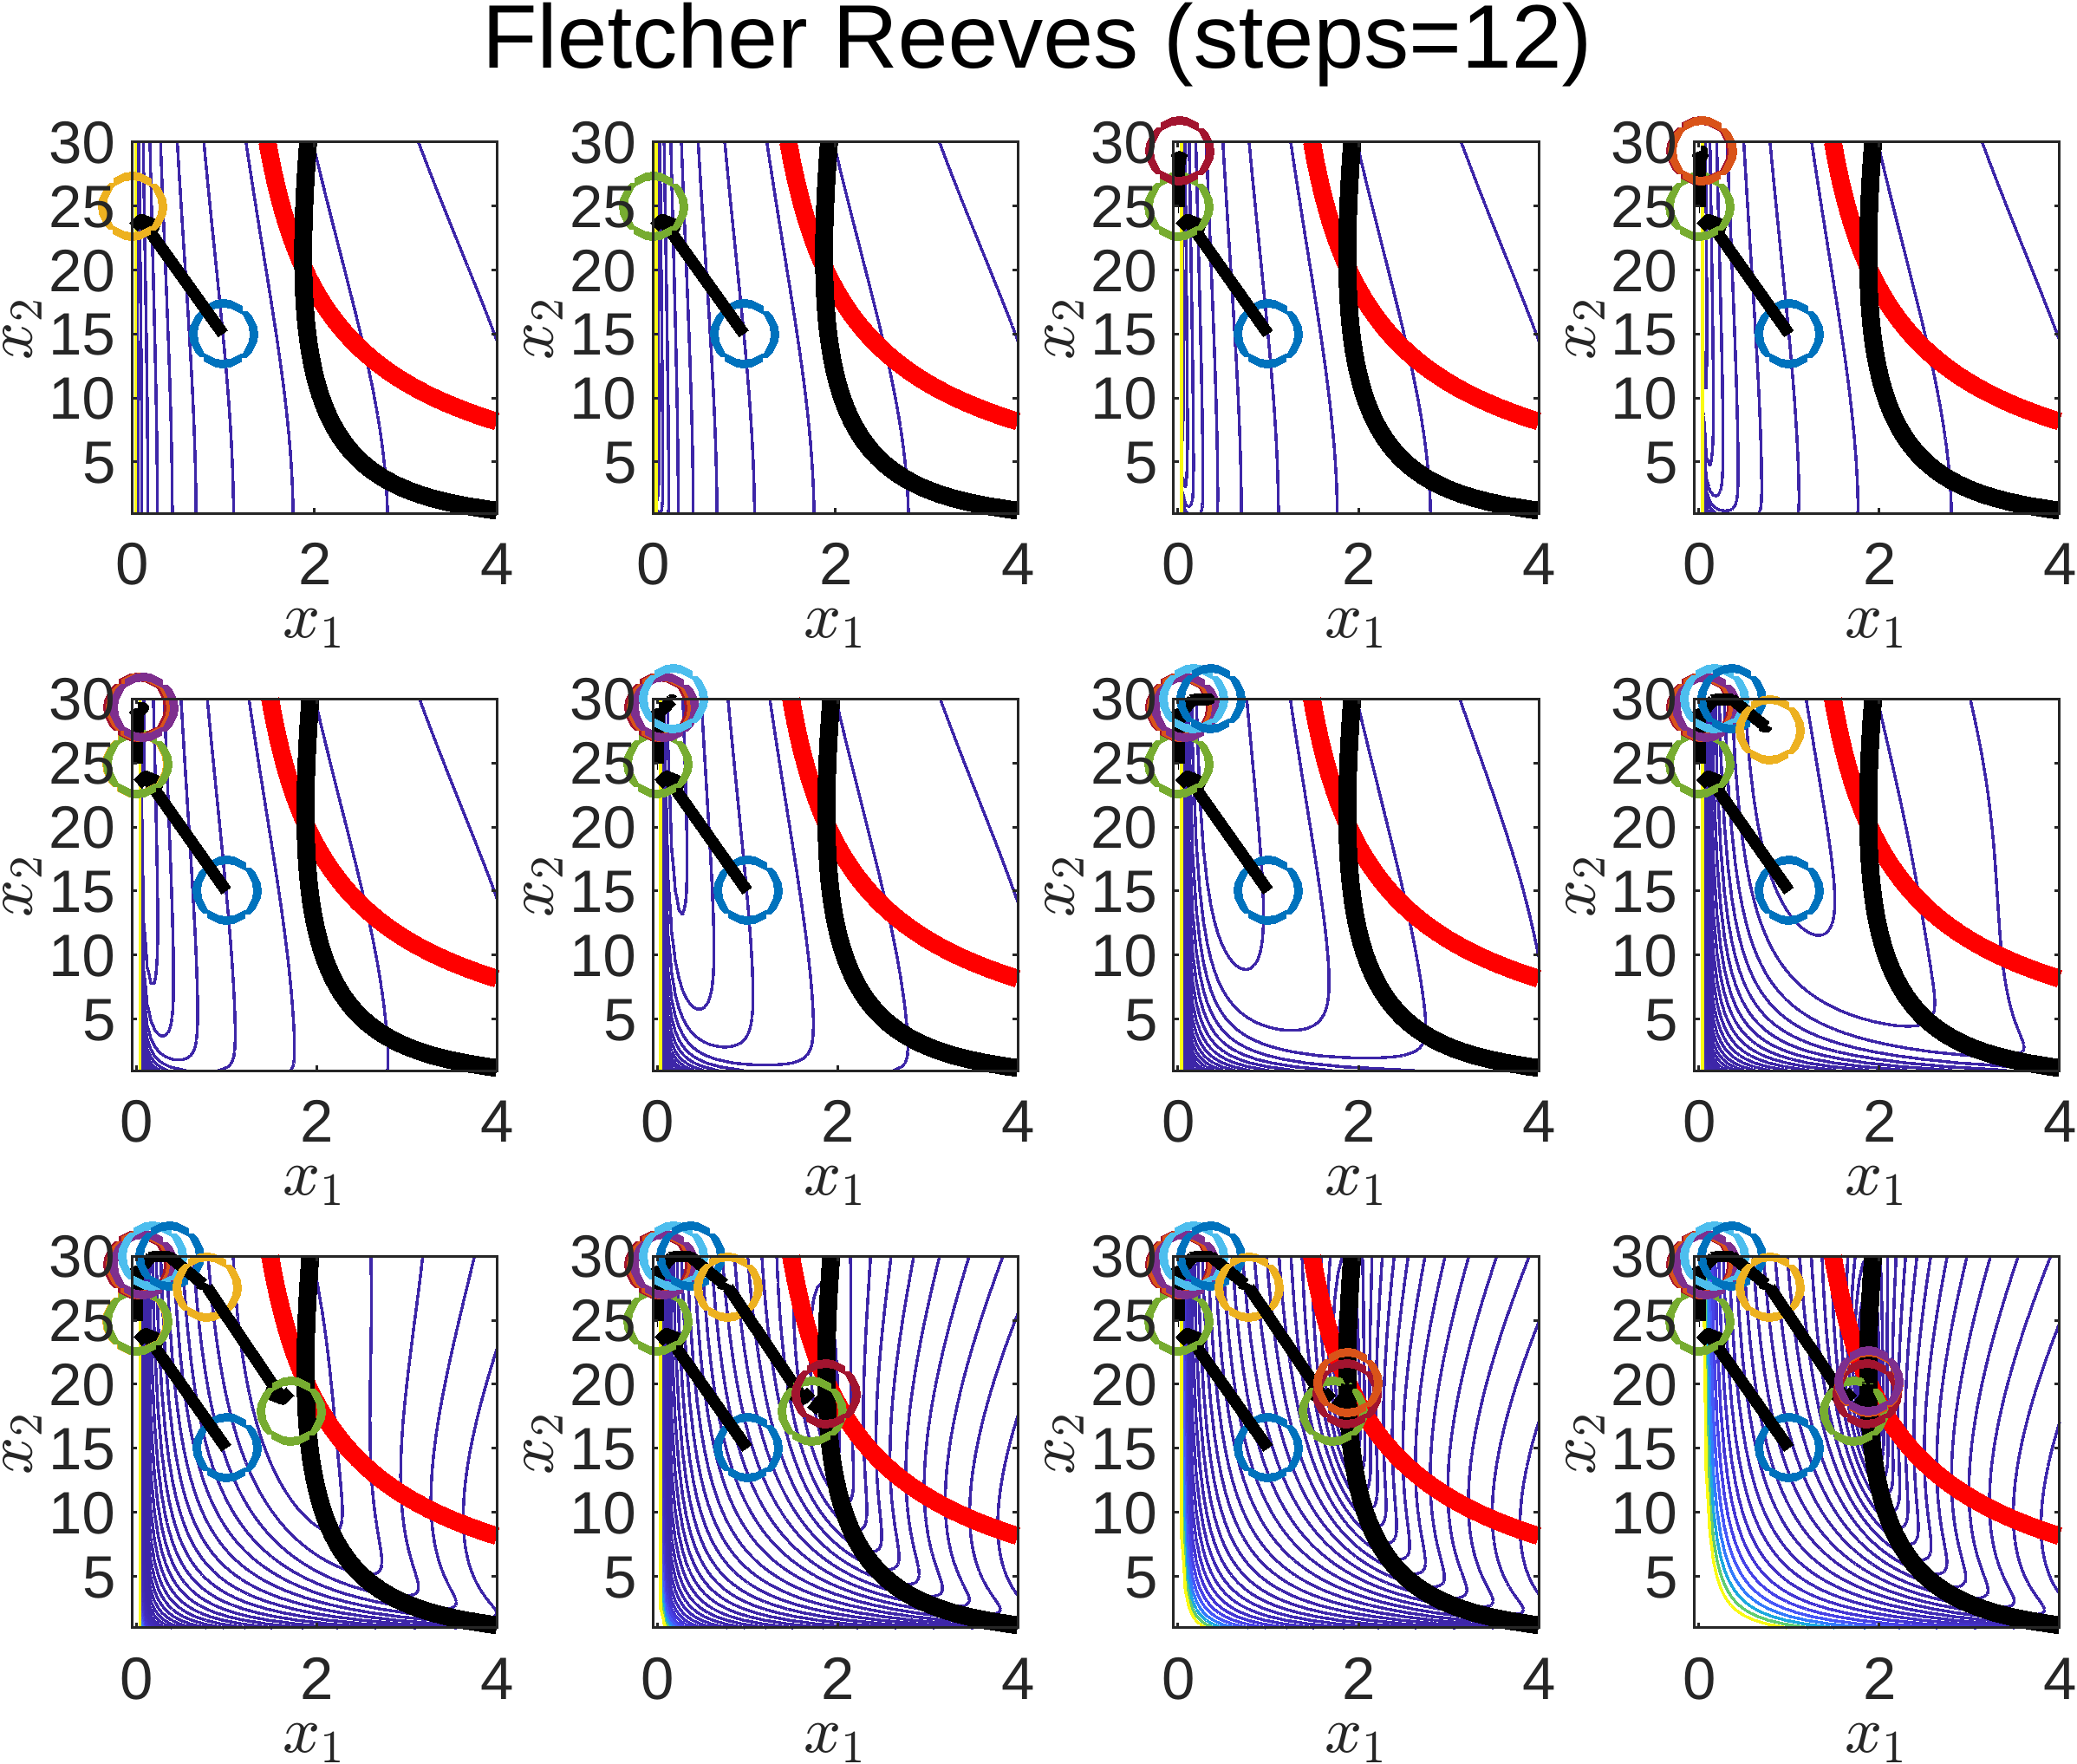
\includegraphics[width=0.8\textwidth]{fig05_P02_PEN_X1_FR.png}
      \caption{OCR do problema 02 pelo m\'etodo da penalidade, a partir do ponto $x^0=\{1,15\}$ - Algoritmo de Flecher-Reeves}
      \label{fig:fig05}
\end{figure}
\begin{figure}[H]
      \centering
      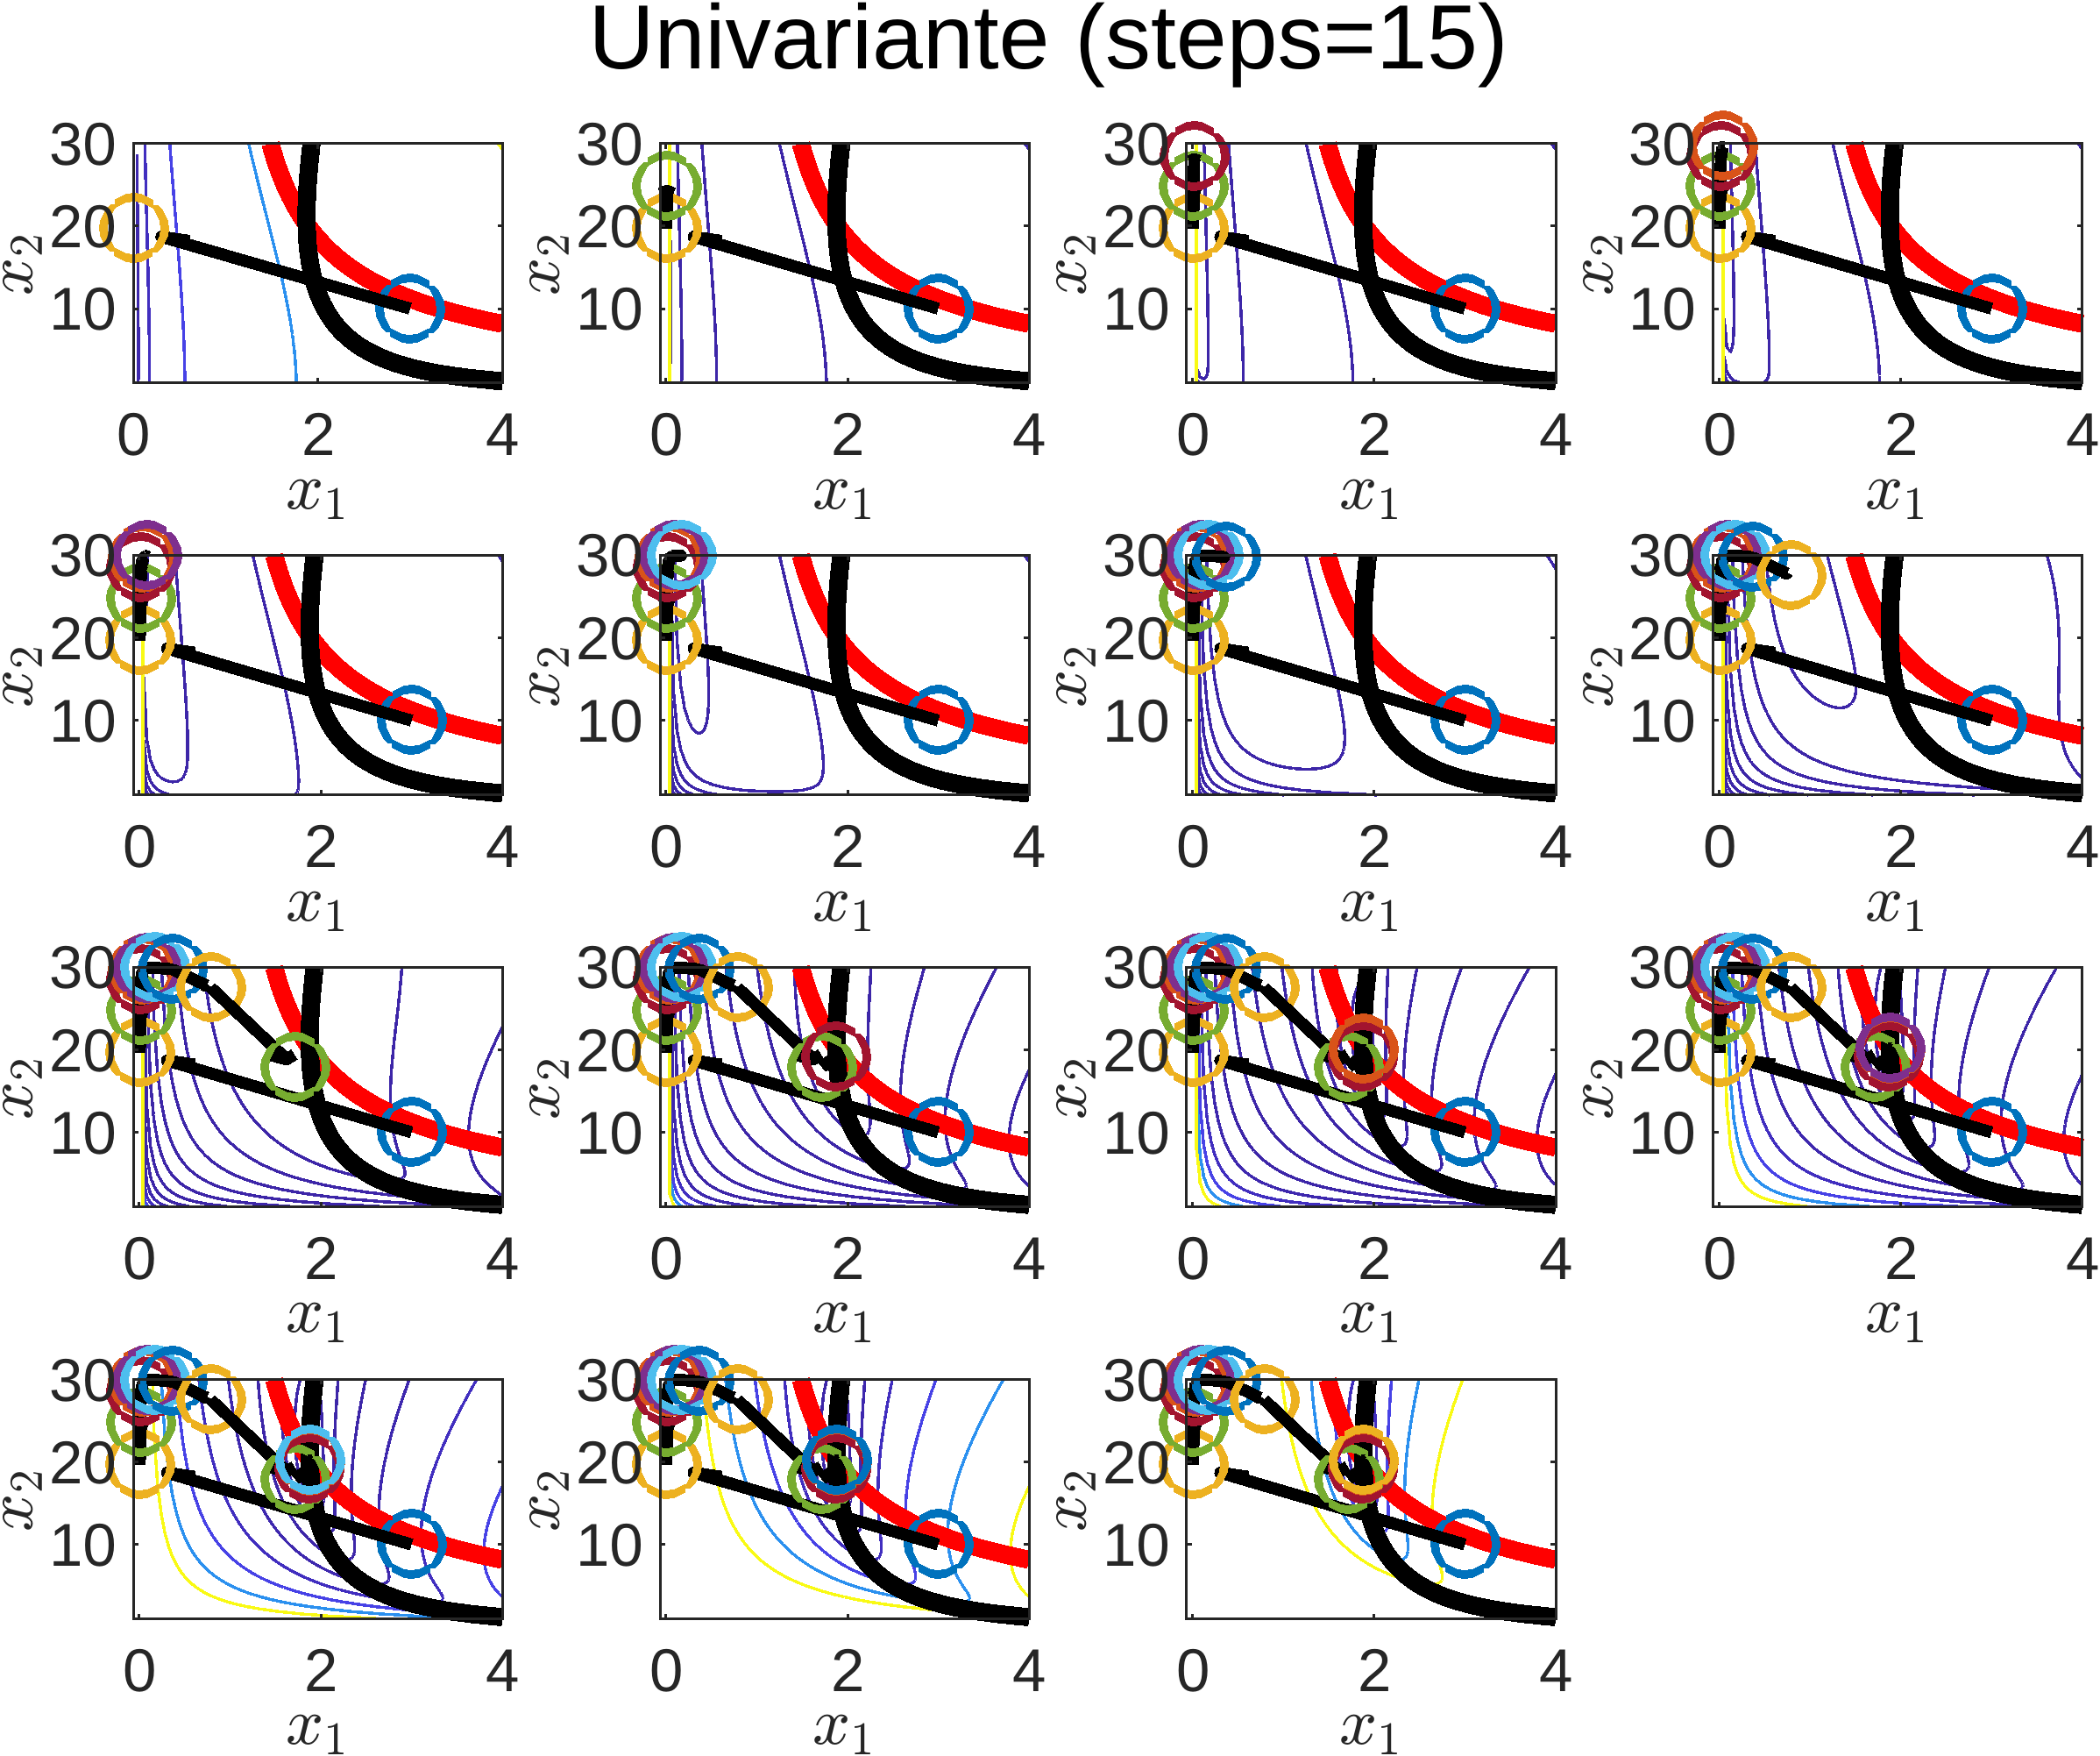
\includegraphics[width=0.8\textwidth]{fig06_P02_PEN_X2_UNI.png}
      \caption{OCR do problema 02 pelo m\'etodo da penalidade, a partir do ponto $x^0=\{3,3\}$ - Algoritmo Univariante}
      \label{fig:fig06}
\end{figure}

Nas figuras \ref{fig:fig07} e \ref{fig:fig08} a seguir ilustra-se as converg\^encias do algoritmo de OCR pelo m\'etodo de barreira para dois pontos de partida distintos: $x^0=\{4,25\}$ e $x^0=\{10,5\}$, respecivamente. O primeiro utilizando, para OSR o m\'etodo de dire\c c\~oes de busca de Newton-Raphson e o segundo, Fletcher-Reeves.

\begin{figure}[H]
      \centering
      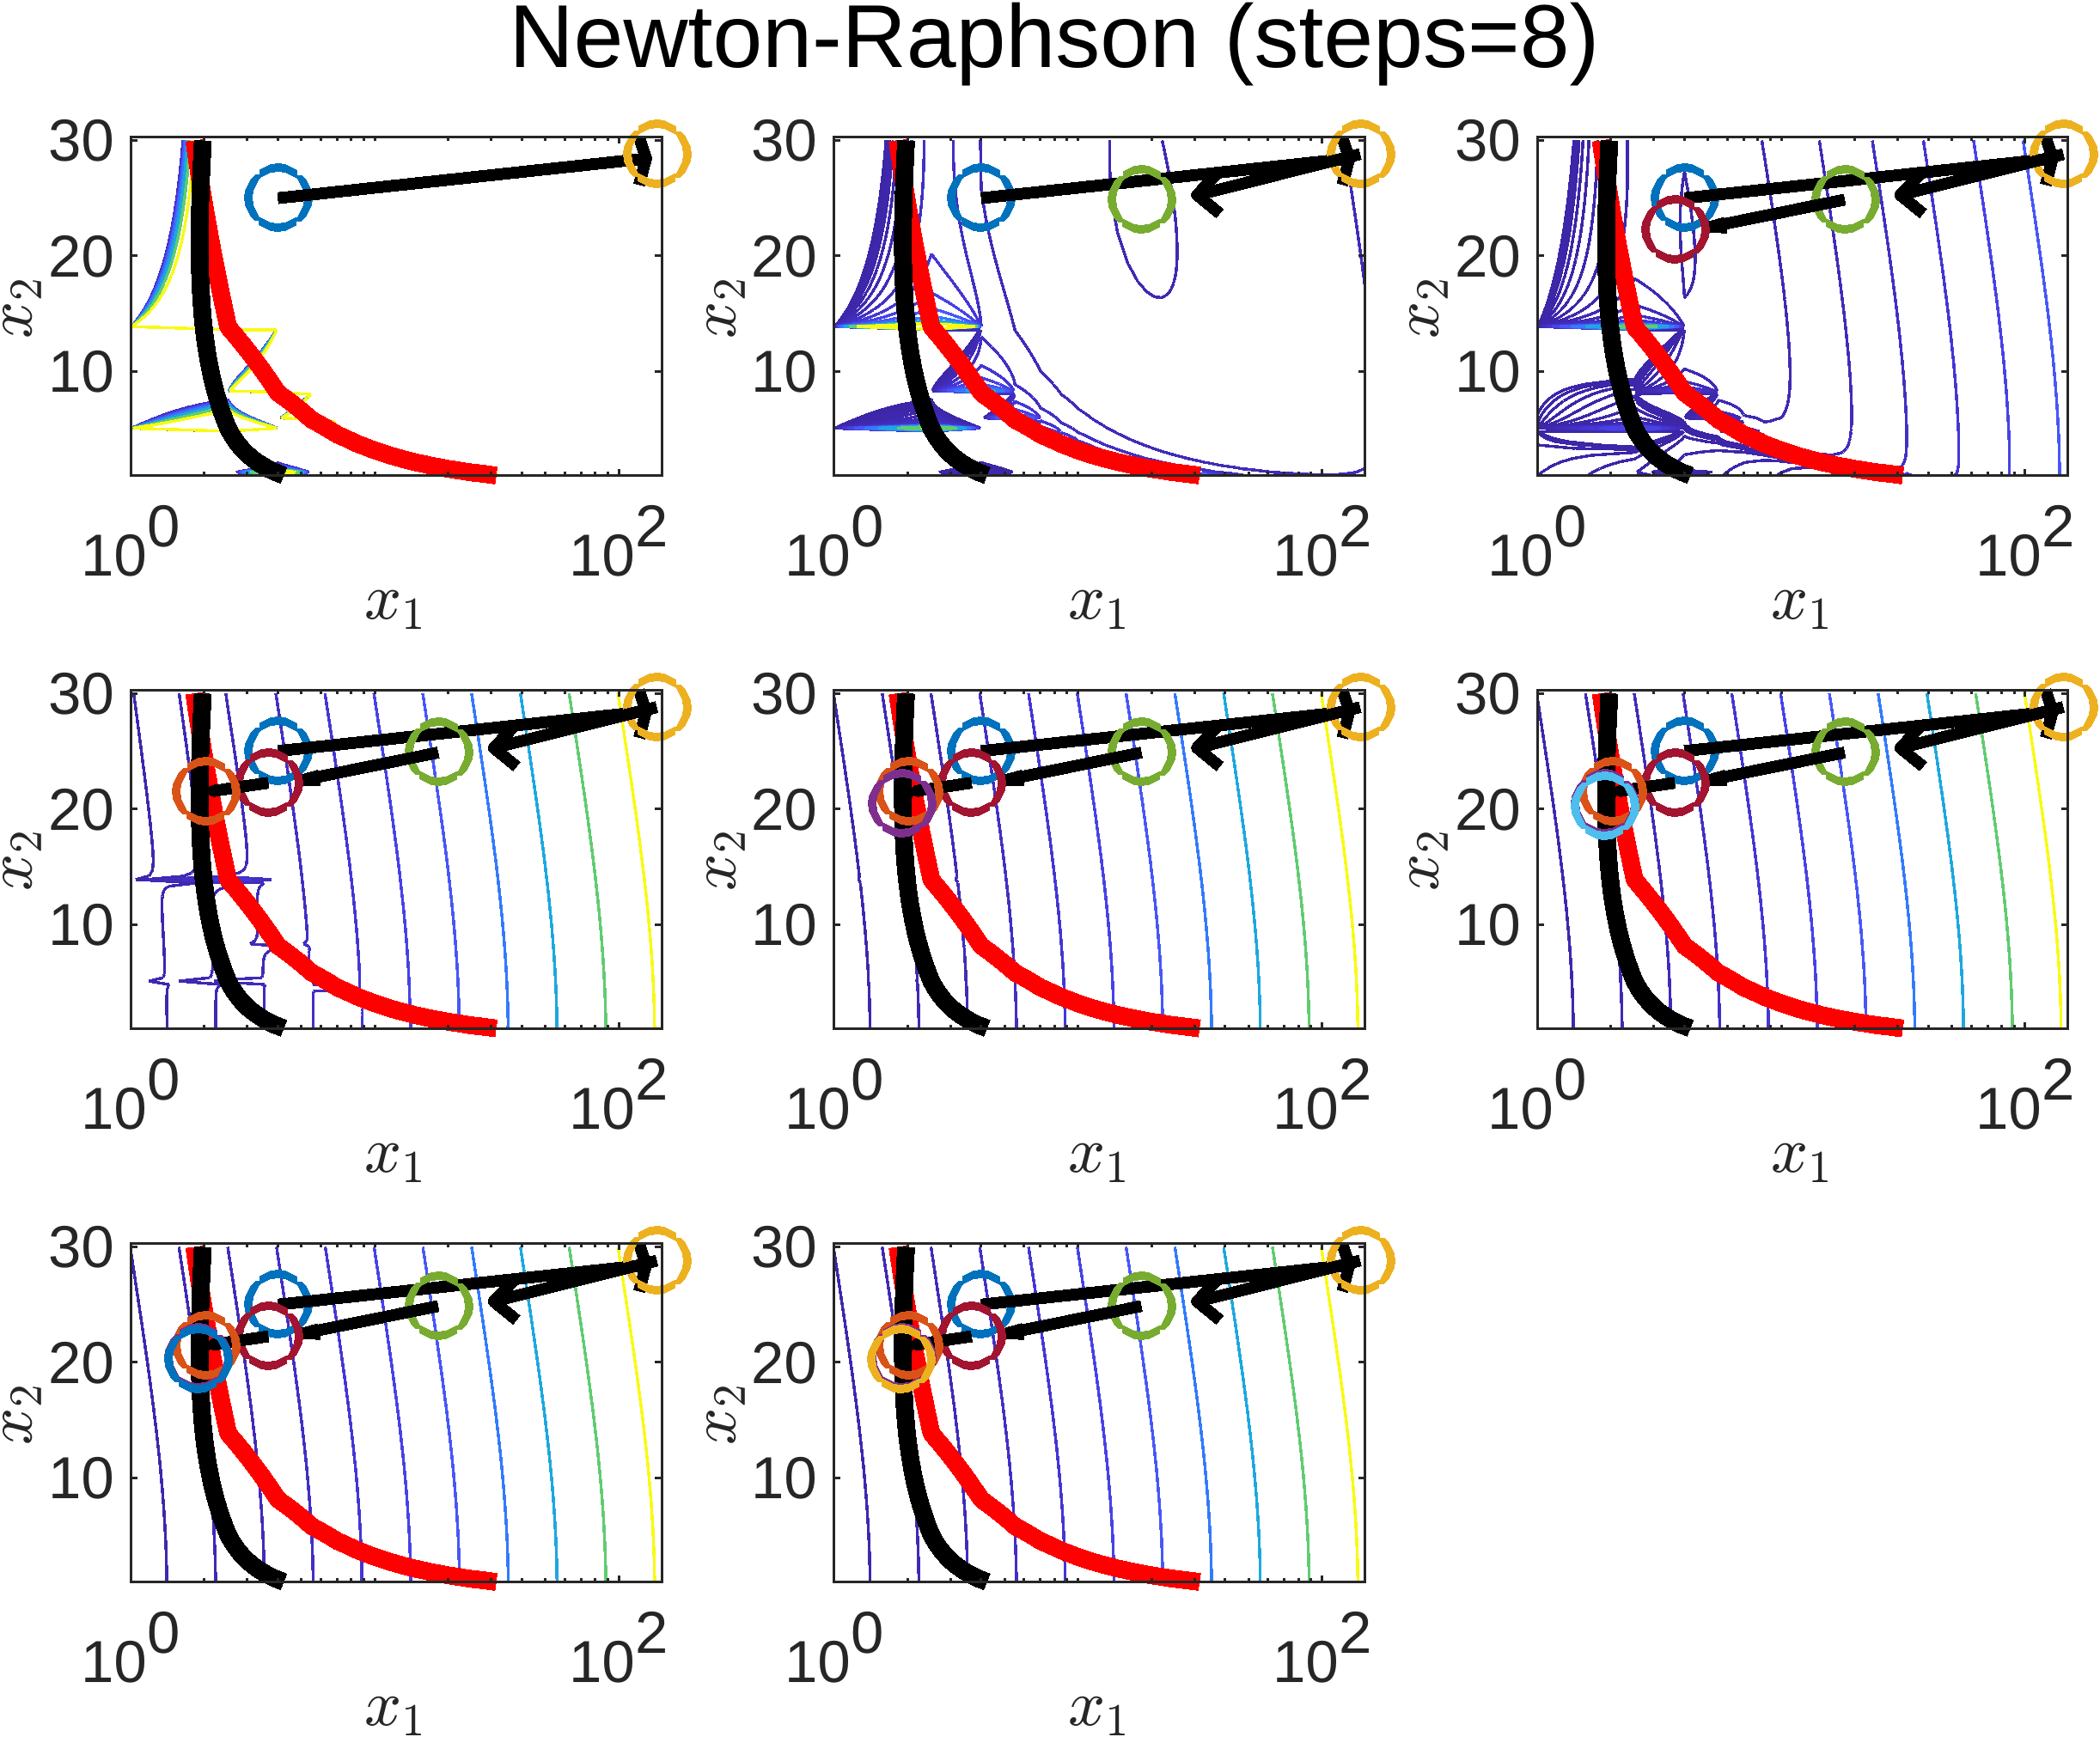
\includegraphics[width=0.7\textwidth]{fig07_P02_BAR_X1_NR.png}
      \caption{OCR do problema 02 pelo m\'etodo da barreira, a partir do ponto $x^0=\{4,25\}$ - Algoritmo de Newton-Raphson}
      \label{fig:fig07}
\end{figure}
\begin{figure}[H]
      \centering
      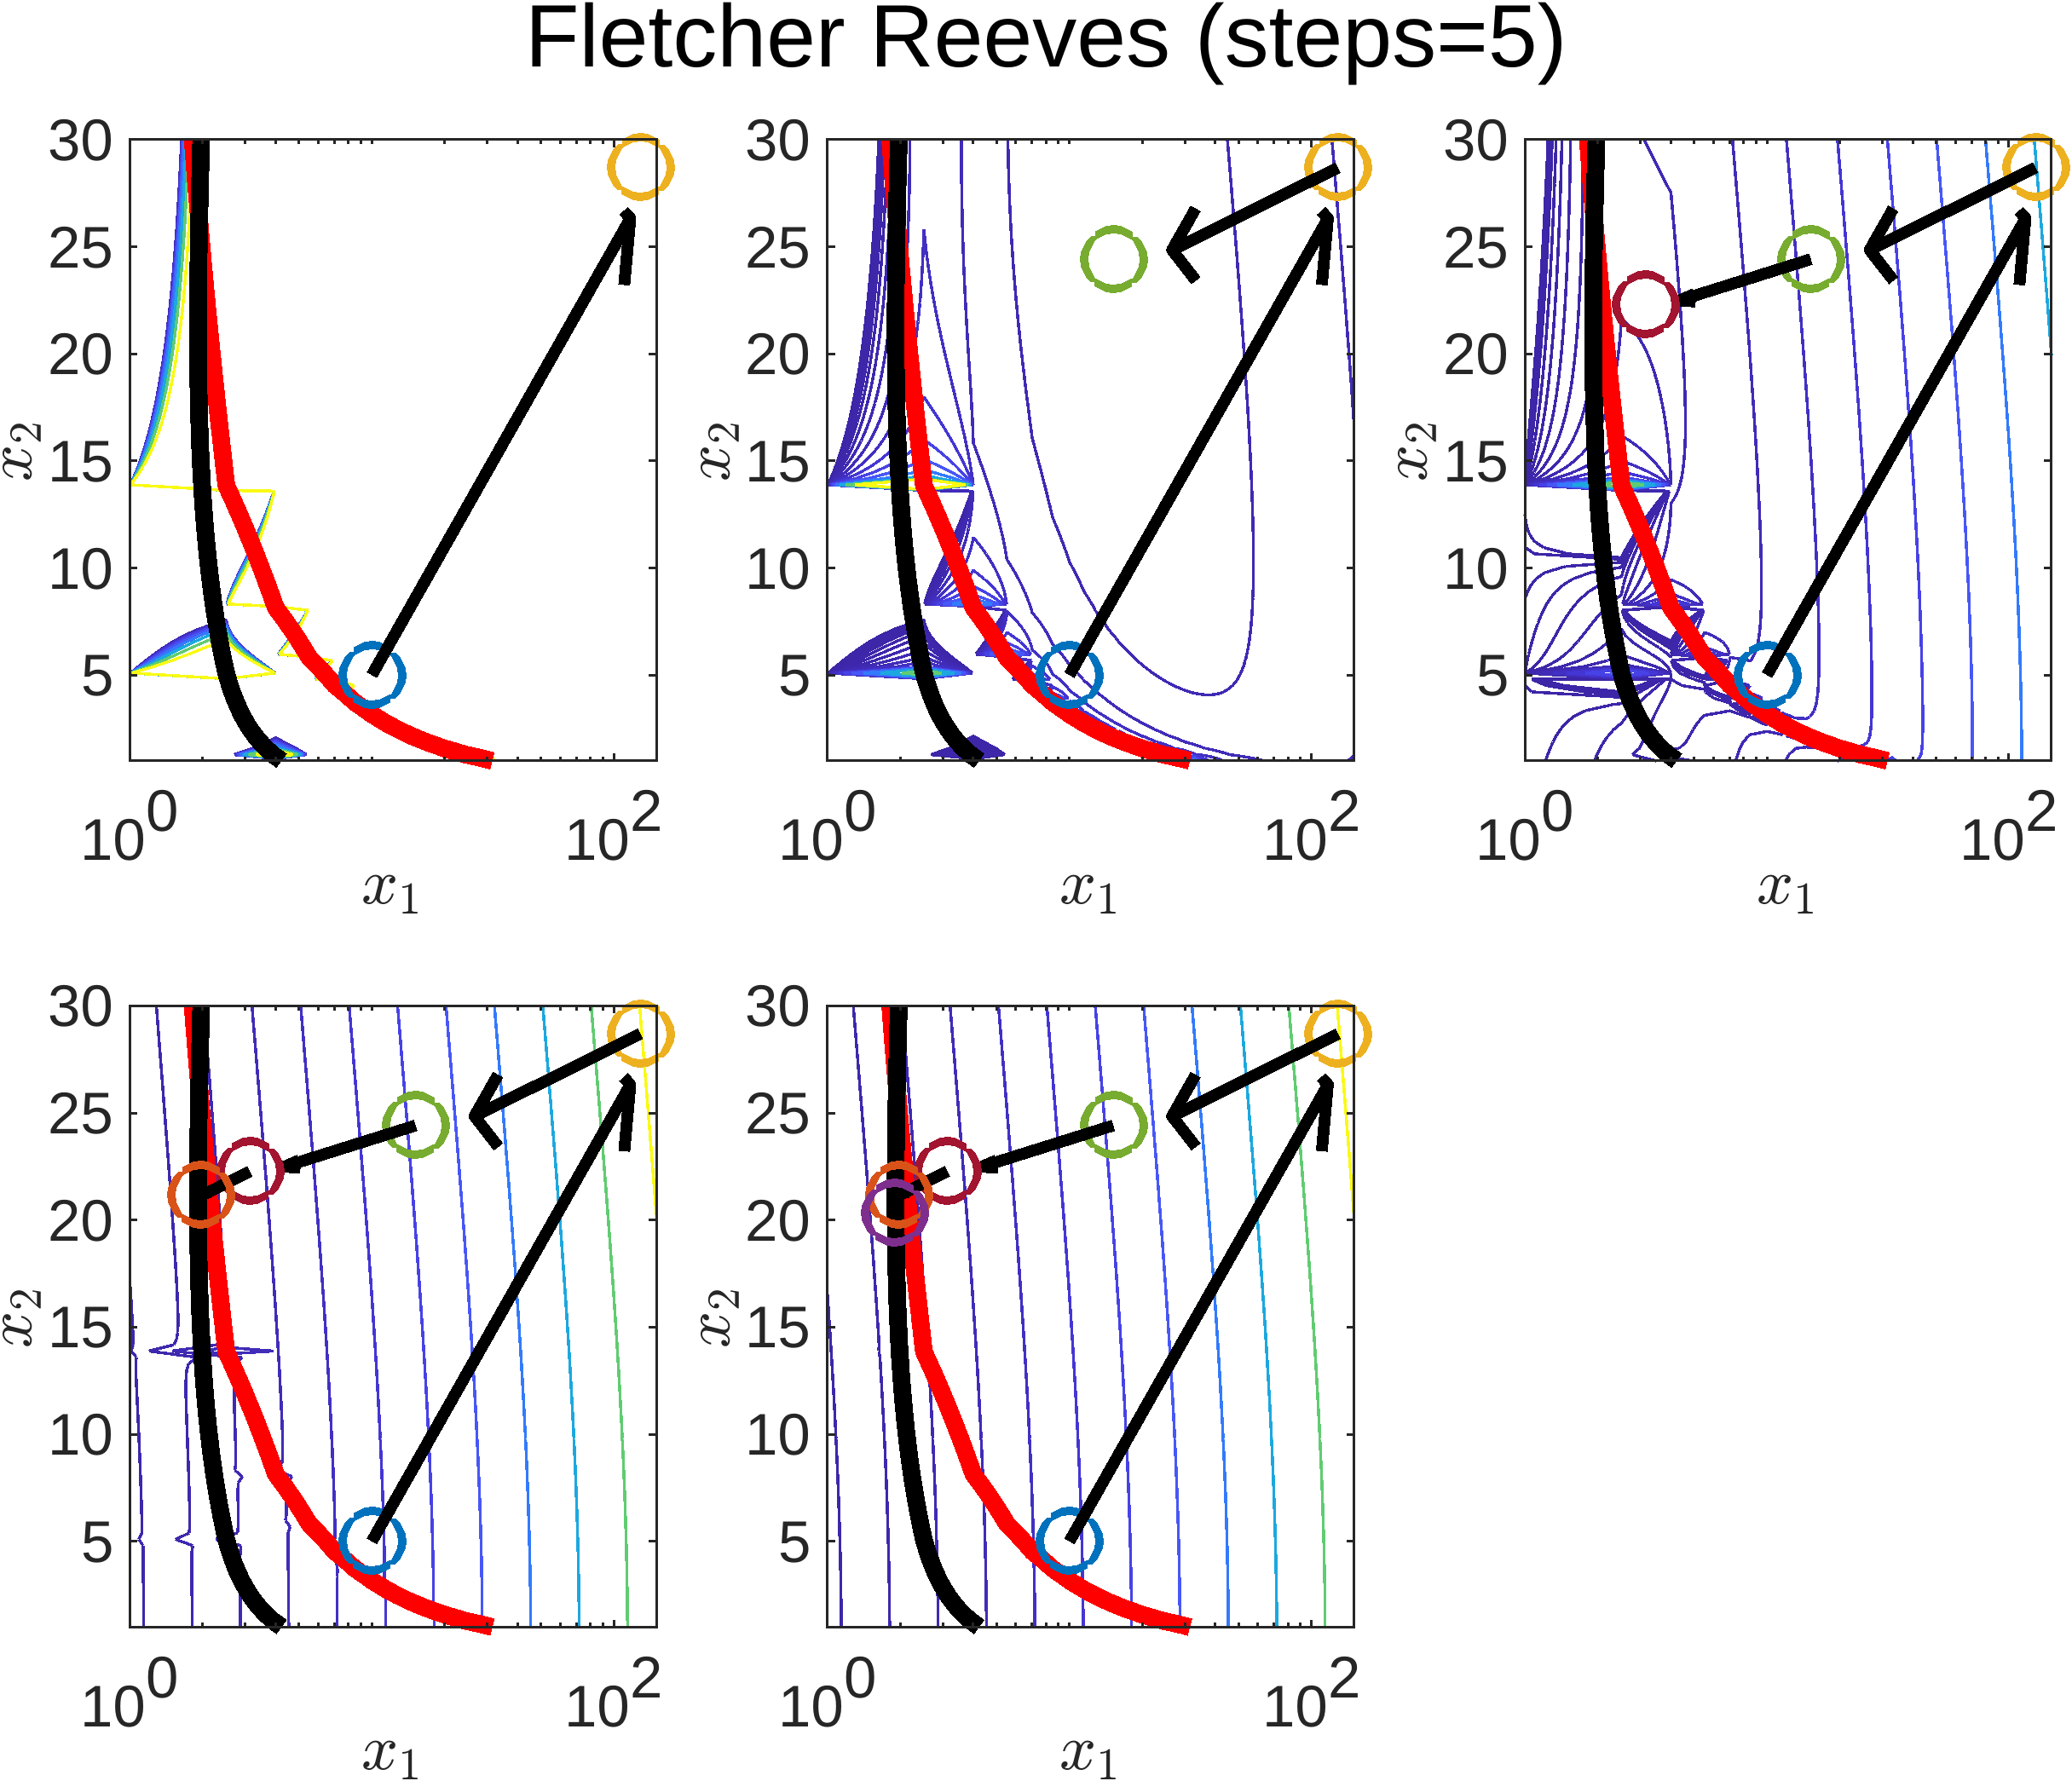
\includegraphics[width=0.7\textwidth]{fig08_P02_BAR_X2_FR.png}
      \caption{OCR do problema 02 pelo m\'etodo da barreira, a partir do ponto $x^0=\{10,5\}$ - Algoritmo de Fletcher-Reeves}
      \label{fig:fig08}
\end{figure}

\section{Conclus\~oes}

A realiza\c c\~ao deste trabalho permitiu implementar os m\'etodos indiretos de solu\c c\~ao de problemas de otimiza\c c\~ao com restri\c c\~ao (OCR) estudados na disciplina de otimiza\c c\~ao. Para todos os casos de aplica\c c\~ao, foram rodados os algortimos para outros pontos que n\~ao os pontos propostos no problema em si e cujo resultado mostrou que os algortimos de busca e miniza\c c\~ao s\~ao robustos.

Devido \`as inefici\^encias do m\'etodo de busca linear e a maior complexidade da pseudo-fun\c c\~ao objetivo a partir da incorpora\c c\~ao dos termos de penalidade, foi necess\'ario ajustar os par\^ametros dos algoritmos para se obter a converg\^encia.

No problema 02, dadas as constantes f\'isicas associadas ao problema, que impuseram \`as fun\c c\~oes alguns termos com n\'umeros grandes, foi fundamental a normaliza\c c\~ao das restri\c c\~oes para sua converg\^encia.

Em geral, notou-se que a converg\^encia, n\'umero de passos e o tempo de execu\c c\~ao dos algoritmos \'e muito sens\'ivel a escolha de seus par\^metros, o que reside nas incertezas num\'ericas associadas aos m\'etodos de busca linear, principalmente.

Apesar da solu\c cao do problema de OSR para algumas configura\c c\~oes da fun\c c\~ao $\phi$ n\~ao ter convergido em alguns passos, a melhor solu\c c\~ao aproximada at\'e o n\'umero m\'aximo de itera\c c\~oes foi suficiente para a converg\^encia geral do problema de OCR.

\section{Anexos}

A seguir est\~ao ilustrados alguns dos c\'odigos ou trechos de c\'odigos decritos na se\c c\~ao metodologia.

\begin{minipage}{\linewidth}
      \begin{lstlisting}[style=myStyle, caption=Inicializa\c c\~ao e dados do problema 01, label=list_prob01]
            % parametros dos algoritmos
            iter_max = 500;
            methods = ["Univariante","Powell","Steepest Descent","Fletcher Reeves","Newton-Raphson","BFGS"];

            % dados do item 01
            f1 = @(x) (x(1)-2)^4 + (x(1)-2*x(2))^2;
            gf1 = @(x) [2*(2*(x(1)-2)^3 + x(1) - 2*x(2)); 8*x(2)-4*x(1)];
            c1 = @(x) x(1)^2 - x(2);
      \end{lstlisting}
\end{minipage}

\begin{minipage}{\linewidth}
      \begin{lstlisting}[style=myStyle, caption= defini\c c\~ao das fun\c c\~oes e restri\c c\~oes do problema 02, label=list_prob02]
            % dados do item 02
            % ro = 0.3;
            % B = 30;
            % P = 33e3;
            % t = 0.1;
            % E = 3e7;
            % sy = 1e5;
            % f2 = @(x) 2*ro*pi()*x(1)*t*sqrt(x(2)^2+B^2);
            f2 = @(x) 0.1885*x(1)*sqrt(x(2)^2+900);
            c2a = @(x) 1.0504*sqrt(x(2)^2+900)/(x(1)*x(2)) - 1;
            c2b = @(x) 1.0504*sqrt(x(2)^2+900)/(x(1)*x(2)) - 3.7011e2*(x(1)^2+0.01)/(x(2)^2+900);
      \end{lstlisting}
\end{minipage}

\begin{minipage}{\linewidth}
      \begin{lstlisting}[style=myStyle, caption= trecho de c\'odigo do problema 01 (penalidade), label=list_p01_pen]
            fprintf('************* PROBLEMA 01 - PENALIDADE *********************\n');
            x0 = [3;2];
            %x0 = [0;4]; % ponto alternativo
            alphas =    [0.002, 0.002, 0.002, 0.001, 0.05, 0.04];
            bs =        [5, 10, 5, 5, 20, 10];
            TOLS =      [1e-4, 1e-4, 1e-4, 1e-4, 1e-4, 1e-5];
            TOLS2 =     [1e-6, 1e-5, 1e-9, 1e-7, 1e-7, 1e-8];
            plot_model = 0; %escolher qual metodo sera plotado

            if plot_model ~= 0
                figure
                i=3;
                j=3;
            end
            for m = [1:6]
                k=0;
                x=x0;
                x_values = x;
                rp=0.1;

                tstart = tic;
                fprintf('---%s---\n', methods(m));

                while k < iter_max
                    if c1(x) < 0
                        a = 0;
                    else
                        a = 1;
                    end
                    rp = bs(m)*rp;

                    p1 = @(x) a * c1(x)^2;
                    phi1 = @(x) f1(x) + 1/2 * rp * p1(x);
                    gphi1 = @(x) [2*(a*rp*x(1)*(x(1)^2-x(2))+2*(x(1)-2)^3+x(1)-2*x(2)); -a*rp*x(1)^2+x(2)*(a*rp+8)-4*x(1)];
                    hess1 = @(x) ...
                        [[2*a*rp*(x(1)^2-x(2)) + 4*a*rp*x(1)^2 + 12*(x(1) - 2)^2 + 2, -2*a*rp*x(1) - 4];
                        [-2*a*rp*x(1) - 4, a*rp + 8]];

                    [x_] = osr_noprint(phi1, gphi1, hess1, x, m, iter_max, alphas(m), TOLS(m), TOLS2(m));
                    k=k+1;

                    if 1/2*p1(x)*rp < TOLS(m)*10 && p1(x) ~= 0
                        conv=1;
                        fprintf('x=[%.4f,%.4f], f(x)=%.4f (%d iter/%.1fms)\n', x(1), x(2), f1(x), k-1, toc(tstart)*1000);
                        break;
                    end
                    x = x_(:,end);
                    x_values = [x_values,x];

                    intervals = [0 1 2 5 10 25 100:500:10000];
                    if m == plot_model
                        phi1_plot = @(x1,x2) (x1-2).^4 + (x1-2*x2).^2+1/2*a*rp*(x1.^2-x2).^2;
                        c_plot = @(x1) x1.^2;
                        intervals = intervals*10;
                        tit = strcat(methods(m), ' (k=',num2str(k),')');
                        plot_phi(-3, 3, 0, 9, phi1_plot, intervals, c_plot, x_values, tit, k, i, j);
                    end
                end
                            if ~conv
                    fprintf('\n nao deu');
                end
            end
      \end{lstlisting}
\end{minipage}


\begin{minipage}{\linewidth}
      \begin{lstlisting}[style=myStyle, caption= trecho de c\'odigo do problema 01 (barreira), label=list_p01_bar]
            fprintf('************* PROBLEMA 01 - BARREIRA *********************\n');
            x0 = [0;1];
            %x0 = [2.5;10]; % ponto alternativo
            alphas =    [0.0002, 0.0002, 0.0002, 0.0002, 0.002, 0.0002];
            bs =        [0.05,      0.2,    0.05, 0.05, 0.05, 0.05];
            TOLS =      [2e-4,      6e-4,   2e-4, 2e-4, 1e-6, 2e-4];
            TOLS2 =     [1e-8,      1e-5,   1e-7, 1e-7, 1e-7, 1e-5];
            plot_model = 0;

            if plot_model ~= 0
            figure
            i=2;
            j=3;
            end
            for m = [1:6]
            k=0;
            x=x0;
            x_values = x;
            rb=100;

            tstart = tic;
            fprintf('---%s---\n', methods(m));

            while k < iter_max
                  rb = bs(m)*rb;
                  b1 = @(x) - c1(x)^(-1);
                  phib1 = @(x) f1(x) + rb * b1(x); % (x-2)^4 + (x-2y)^2 - a/(x^2-y)

                  gphib1 = @(x) ... % (2 ((a x)/(x^2 - y)^2 + 2 (x - 2)^3 + x - 2 y), -a/(x^2 - y)^2 - 4 x + 8 y)
                        [2*((rb*x(1))/(x(1)^2-x(2))^2 + 2*(x(1)-2)^3 + x(1)-2*x(2)); ...
                        -rb/(x(1)^2-x(2))^2 - 4*x(1)+8*x(2)];

                  hessb1 = @(x) ...
                        [[2 + 12*(-2 + x(1))^2 - (8*rb*x(1)^2)/(x(1)^2 - x(2))^3 + (2*rb)/(x(1)^2 - x(2))^2, -4 + (4*rb*x(1))/(x(1)^2 - x(2))^3]; ...
                        [-4 + (4*rb*x(1))/(x(1)^2 - x(2))^3, 8 - (2*rb)/(x(1)^2 - x(2))^3]];

                  [x_] = osr_noprint(phib1, gphib1, hessb1, x, m, iter_max, alphas(m), TOLS(m), TOLS2(m));

                  b1(x)*rb;
                  if b1(x)*rb < TOLS(m)
                        conv=1;
                        c1(x);
                        fprintf('x=[%.4f,%.4f], f(x)=%.4f (%d iter/%.1fms)\n', x(1), x(2), f1(x), k, toc(tstart)*1000);
                        break;
                  end
                  x = x_(:,end);
                  x_values = [x_values,x];

                  k=k+1;

                  intervals = 10.^[-2:.5:5];
                  if m == plot_model
                        phib1_plot = @(x1,x2) (x1-2).^4 + (x1-2*x2).^2 - rb./(x1.^2-x2);
                        c_plot = @(x1) x1.^2;
                        tit = strcat(methods(m), ' (k=',num2str(k),')');
                        plot_phi(-2, 2, 0, 4, phib1_plot, intervals, c_plot, x_values, tit, k, i , j);
                  end
            end

            if ~conv
                  fprintf('\n nao deu');
            end
      \end{lstlisting}
\end{minipage}


\begin{minipage}{\linewidth}
      \begin{lstlisting}[style=myStyle, caption= trecho de c\'odigo do problema 02 (penalidade) (1/2), label=list_p02_pen_1]
            x0 = [1;15];
            %x0 = [3;3]; %ponto alternativo
            alphas =    [0.005, 0.005, 0.0001,  0.0001, 0.0002, 0.0002];
            bs =        [10,    50,      10,    10,     10,       10];
            TOLS =      [1e-6,  1e-6,   2e-3,   1e-3,   1e-5,   5e-3];
            TOLS_OCR =  [1e-6,  1e-6,   1e-4,   5e-4,   1e-6,   1e-4];
            TOLS2 =     [1e-7,  1e-5,   1e-7,   1e-7,   1e-7,   1e-7];
            plot_model = 0;

            if plot_model ~= 0
            figure
            i=4;
            j=4;
            end
            for m = [1:6]
            k=0;
            x=x0;
            x_values = x;
            rp=1e-8;

            tstart = tic;
            fprintf('---%s---\n', methods(m));

            while k < 20
                  if c2a(x) < 0
                        a(1) = 0;
                  else
                        a(1) = 1;
                  end
                  if c2b(x) < 0
                        a(2) = 0;
                  else
                        a(2) = 1;
                  end

                  rp = bs(m)*rp;
                  p2 = @(x) a(1) * c2a(x)^2 + a(2) * c2b(x)^2;
                  phi2 = @(x) f2(x) + 1/2 * rp * p2(x);

                  g2f = @(x) ...
                  [0.1885*sqrt(x(2)^2+900);
                  (0.1885*x(1)*x(2))/sqrt(x(2)^2+900)];
                  g2c1 = @(x) ...
                  [(a(1)*rp*(1.0504*x(1)*sqrt(x(2)^2+900)*x(2)-1.10334*x(2)^2-993.006))/(x(1)^3*x(2)^2);
                  (a(1)*rp*((945.36*x(1)*x(2))/sqrt(x(2)^2+900)-993.006))/(x(1)^2*x(2)^3)];
                  g2c2 = @(x) ...
                  [a(2)*rp*(-(1.0504*sqrt(x(2)^2 + 900))/(x(1)^2*x(2)) - (740.22*x(1))/(x(2)^2 + 900))*((1.0504*sqrt(x(2)^2 + 900))/(x(1)*x(2)) - (370.11*(x(1)^2 + 0.01))/(x(2)^2 + 900));
                  a(2)*rp*((740.22*x(1)^2*x(2))/(x(2)^2 + 900)^2 - 945.36/(x(1)*x(2)^2*sqrt(x(2)^2 + 900)) + (7.4022*x(2))/(x(2)^2 + 900)^2)*((1.0504*sqrt(x(2)^2 + 900))/(x(1)*x(2)) - (370.11*(x(1)^2 + 0.01))/(x(2)^2 + 900))];

                  gphi2 = @(x) g2f(x)+g2c1(x)+g2c2(x);

                  hess2 = @(x) ...
                        [[(1.10334*a(1)*rp*(900 + x(2)^2))/(x(1)^4*x(2)^2) + a(2)*rp*((-740.22*x(1))/(900 + x(2)^2) - (1.0504*sqrt(900 + x(2)^2))/(x(1)^2*x(2)))^2 + (2.1008*a(1)*rp*sqrt(900 + x(2)^2)*(-1 + (1.0504*sqrt(900 + x(2)^2))/(x(1)*x(2))))/(x(1)^3*x(2)) + a(2)*rp*(-740.22/(900 + x(2)^2) + (2.1008*sqrt(900 + x(2)^2))/(x(1)^3*x(2)))*((-370.11*(0.01 + x(1)^2))/(900 + x(2)^2) + (1.0504*sqrt(900 + x(2)^2))/(x(1)*x(2))), ...
      \end{lstlisting}
\end{minipage}

\begin{minipage}{\linewidth}
      \begin{lstlisting}[style=myStyle, caption= trecho de c\'odigo do problema 02 (penalidade) (2/2), label=list_p02_pen_2]
                        (0.1885*x(2))/sqrt(900 + x(2)^2) - (1.0504*a(1)*rp*sqrt(900 + x(2)^2)*(1.0504/(x(1)*sqrt(900 + x(2)^2)) - (1.0504*sqrt(900 + x(2)^2))/(x(1)*x(2)^2)))/(x(1)^2*x(2)) + a(2)*rp*((740.22* (0.01 + x(1)^2)*x(2))/(900 + x(2)^2)^2 + 1.0504/(x(1)*sqrt(900 + x(2)^2)) - (1.0504*sqrt(900 + x(2)^2))/(x(1)*x(2)^2))*((-740.22*x(1))/(900 + x(2)^2) - (1.0504*sqrt(900 + x(2)^2))/(x(1)^2*x(2))) - (1.0504*a(1)*rp*(-1 + (1.0504*sqrt(900 + x(2)^2))/(x(1)*x(2))))/(x(1)^2*sqrt(900 + x(2)^2)) + (1.0504*a(1)*rp*sqrt(900 + x(2)^2)*(-1 + (1.0504*sqrt(900 + x(2)^2))/(x(1)*x(2))))/(x(1)^2*x(2)^2) + a(2)*rp*((1480.44*x(1)*x(2))/(900 + x(2)^2)^2 - 1.0504/(x(1)^2*sqrt(900 + x(2)^2)) + (1.0504*sqrt(900 + x(2)^2))/(x(1)^2*x(2)^2))* ((-370.11*(0.01 + x(1)^2))/(900 + x(2)^2) + (1.0504*sqrt(900 + x(2)^2))/(x(1)*x(2)))]; ...
                        [(0.1885*x(2))/sqrt(900 + x(2)^2) - (1.0504*a(1)*rp*sqrt(900 + x(2)^2)*(1.0504/(x(1)*sqrt(900 + x(2)^2)) - (1.0504*sqrt(900 + x(2)^2))/(x(1)*x(2)^2)))/(x(1)^2*x(2)) + a(2)*rp*((740.22* (0.01 + x(1)^2)*x(2))/(900 + x(2)^2)^2 + 1.0504/(x(1)*sqrt(900 + x(2)^2)) - (1.0504*sqrt(900 + x(2)^2))/(x(1)*x(2)^2))*((-740.22*x(1))/(900 + x(2)^2) - (1.0504*sqrt(900 + x(2)^2))/(x(1)^2*x(2))) - (1.0504*a(1)*rp*(-1 + (1.0504*sqrt(900 + x(2)^2))/(x(1)*x(2))))/(x(1)^2*sqrt(900 + x(2)^2)) + (1.0504*a(1)*rp*sqrt(900 + x(2)^2)*(-1 + (1.0504*sqrt(900 + x(2)^2))/(x(1)*x(2))))/(x(1)^2*x(2)^2) + a(2)*rp*((1480.44*x(1)*x(2))/(900 + x(2)^2)^2 - 1.0504/(x(1)^2*sqrt(900 + x(2)^2)) + (1.0504*sqrt(900 + x(2)^2))/(x(1)^2*x(2)^2))* ((-370.11*(0.01 + x(1)^2))/(900 + x(2)^2) + (1.0504*sqrt(900 + x(2)^2))/(x(1)*x(2))), ...
                        (-0.1885*x(1)*x(2)^2)/(900 + x(2)^2)^(3/2) + (0.1885*x(1))/sqrt(900 + x(2)^2) + a(1)*rp*(1.0504/(x(1)*sqrt(900 + x(2)^2)) - (1.0504*sqrt(900 + x(2)^2))/(x(1)*x(2)^2))^2 + a(2)*rp*((740.22*(0.01 + x(1)^2)*x(2))/(900 + x(2)^2)^2 + 1.0504/(x(1)*sqrt(900 + x(2)^2)) - (1.0504*sqrt(900 + x(2)^2))/(x(1)*x(2)^2))^2 + a(1)*rp*((-1.0504*x(2))/(x(1)*(900 + x(2)^2)^(3/2)) - 1.0504/(x(1)*x(2)*sqrt(900 + x(2)^2)) + (2.1008*sqrt(900 + x(2)^2))/(x(1)*x(2)^3))*(-1 + (1.0504*sqrt(900 + x(2)^2))/(x(1)*x(2))) + a(2)*rp*((-2960.88*(0.01 + x(1)^2)*x(2)^2)/(900 + x(2)^2)^3 + (740.22*(0.01 + x(1)^2))/(900 + x(2)^2)^2 - (1.0504*x(2))/(x(1)*(900 + x(2)^2)^(3/2)) - 1.0504/(x(1)*x(2)*sqrt(900 + x(2)^2)) + (2.1008*sqrt(900 + x(2)^2))/(x(1)*x(2)^3))*((-370.11*(0.01 + x(1)^2))/(900 + x(2)^2) + (1.0504*sqrt(900 + x(2)^2))/(x(1)*x(2)))]];

                  [x_] = osr_noprint(phi2, gphi2, hess2, x, m, 400, alphas(m), TOLS(m), TOLS2(m));
                  x = x_(:,end);
                  x_values = [x_values,x];
                  k=k+1;

                  if 1/2*p2(x)*rp < TOLS_OCR(m)
                        conv=1;
                        fprintf('x=[%.4f,%.4f], f(x)=%.4f (%d iter/%.1fms)\n', x(1), x(2), f2(x), k-1, toc(tstart)*1000);
                        break;
                  end

                  intervals=10.^[-3:.1:6];
                  if m == plot_model
                        phi2_plot = @(x1,x2) ...
                        0.1885.*x1.*sqrt(x2.^2+900) + ...
                        1/2*rp*a(1)*(1.0504.*sqrt(x2.^2+900)./(x1.*x2) - 1).^2 + ...
                        1/2*rp*a(2)*(1.0504.*sqrt(x2.^2+900)./(x1.*x2) - 3.7011e2.*(x1.^2+0.01)./(x2.^2+900)).^2;
                        c_plot = @(x1) -1;
                        tit = strcat(methods(m), ' (k=',num2str(k),')');
                        plot_phi(0, 4, 1, 100, phi2_plot, intervals, c_plot, x_values, tit, k, i, j);
                  end
            end
            if ~conv
                  fprintf('\n nao deu');
            end
      \end{lstlisting}
\end{minipage}

\begin{minipage}{\linewidth}
      \begin{lstlisting}[style=myStyle, caption= trecho de c\'odigo do problema 02 (barreira) (1/2), label=list_p02_bar_1]
            x0 = [4;25];
            % x0 = [10;5];
            % verifica se o ponto alternativo) esta na regiao viavel
            % c2a(x0)
            % c2b(x0)
            alphas =    [0.0001,  0.0001,  0.00002, 0.00002, 0.001,   0.0002];
            bs =        [  0.12,    0.09,   0.005,   0.008,   0.01,   0.0006];
            TOLS =      [  1e-4,    1e-4,    5e-4,   1e-4,    1e-6,    1e-5];
            TOLS_OCR =  [  2e-4,    2e-4,    2e-4,   3e-4,    1e-6,    1e-4];
            TOLS2 =     [  1e-9,    1e-10,   1e-9,   1e-7,    1e-6,    1e-8];
            plot_model = 0;

            if plot_model ~= 0
                figure
                i=3;
                j=2;
            end
            for m = [1:6]
                k=0;
                x=x0;
                x_values = x;
                rb=1e7;

                tstart = tic;
                fprintf('---%s---\n', methods(m));

                while k < iter_max
                  rb = bs(m)*rb;
                  b2 = @(x) -c2a(x)^-1 -c2b(x)^-1;
                  phib2 = @(x) f2(x) + rb * b2(x);

                  g2f = @(x) ...
                  [0.1885*sqrt(x(2)^2+900);
                  (0.1885*x(1)*x(2))/sqrt(x(2)^2+900)];

                  g2c1 = @(x) ...
                  [-(0.952018*rb*x(2)*sqrt(x(2)^2 + 900))/(0.952018*x(1)*x(2) - sqrt(x(2)^2 + 900))^2;
                  -(856.816*rb*x(1))/(sqrt(x(2)^2 + 900)*(0.952018*x(1)*x(2) - sqrt(x(2)^2 + 900))^2)];

                  g2c2 = @(x) ...
                  [-(0.952018*rb*x(2)*(x(2)^2 + 900)*(704.703*x(1)^3*x(2) + (x(2)^2 + 900)^(3/2)))/(352.351*x(1)^3*x(2) + 3.52351*x(1)*x(2) - (x(2)^2 + 900)^(3/2))^2; ...
                  (670.89*rb*x(1)*((x(1)^3 + 0.01*x(1))*sqrt(x(2)^2 + 900)*x(2)^3 - 1.27713*x(2)^4 - 2298.84*x(2)^2 - 1.03448*10^6))/(sqrt(x(2)^2 + 900)*(352.351*x(1)^3*x(2) + 3.52351*x(1)*x(2) - (x(2)^2 + 900)^(3/2))^2)];

                  gphib2 = @(x) g2f(x)+g2c1(x)+g2c2(x);

                  hessf = @(x) ...
                  [[0, ...
                        (0.1885*x(2))/sqrt(900 + x(2)^2)]; [(0.1885* x(2))/sqrt(900 + x(2)^2), ...
                        (-0.1885* x(1)* x(2)^2)/(900 + x(2)^2)^(3/2) + (0.1885* x(1))/sqrt(900 + x(2)^2)]];

                  hessc1 = @(x) ...
                        [[(-2.20668* rb* (900 + x(2)^2))/(x(1)^4* x(2)^2* (-1 + (1.0504* sqrt(900 + x(2)^2))/(x(1)* x(2)))^3) + (2.1008 *rb *sqrt(900 + x(2)^2))/(x(1)^3* x(2)* (-1 + (1.0504* sqrt(900 + x(2)^2))/(x(1)* x(2)))^2), ...
                        (2.1008 *rb* sqrt(900 + x(2)^2)* (1.0504/(x(1)* sqrt(900 + x(2)^2)) - (1.0504* sqrt(900 + x(2)^2))/(x(1)* x(2)^2)))/(x(1)^2* x(2)* (-1 + (1.0504* sqrt(900 + x(2)^2))/(x(1)* x(2)))^3) - (1.0504 *rb)/(x(1)^2* sqrt(900 + x(2)^2)* (-1 + (1.0504* sqrt(900 + x(2)^2))/(x(1)* x(2)))^2) + (1.0504 *rb* sqrt(900 + x(2)^2))/(x(1)^2* x(2)^2 *(-1 + (1.0504 *sqrt(900 + x(2)^2))/(x(1)* x(2)))^2)];
      \end{lstlisting}
\end{minipage}

\begin{minipage}{\linewidth}
\begin{lstlisting}[style=myStyle, caption= trecho de c\'odigo do problema 02 (barreira) (2/2), label=list_p02_bar_2]
                         [(2.1008 *rb* sqrt(900 + x(2)^2)* (1.0504/(x(1)* sqrt(900 + x(2)^2)) - (1.0504 *sqrt(900 + x(2)^2))/(x(1)* x(2)^2)))/(x(1)^2* x(2)* (-1 + (1.0504 *sqrt(900 + x(2)^2))/(x(1)* x(2)))^3) + (rb* (-1.0504/(x(1)^2 *sqrt(900 + x(2)^2)) + (1.0504* sqrt(900 + x(2)^2))/(x(1)^2* x(2)^2)))/(-1 + (1.0504 *sqrt(900 + x(2)^2))/(x(1)* x(2)))^2, ...
                          (-2* rb* (1.0504/(x(1)* sqrt(900 + x(2)^2)) - (1.0504 *sqrt(900 + x(2)^2))/(x(1)* x(2)^2))^2)/(-1 + (1.0504* sqrt(900 + x(2)^2))/(x(1)* x(2)))^3 + (rb* ((-1.0504 *x(2))/(x(1)* (900 + x(2)^2)^(3/2)) - 1.0504/(x(1) *x(2)* sqrt(900 + x(2)^2)) + (2.1008* sqrt(900 + x(2)^2))/(x(1)* x(2)^3)))/(-1 + (1.0504 *sqrt(900 + x(2)^2))/(x(1)* x(2)))^2]];
                    hessc2 = @(x) ...
                        [[(-2*rb* ((-740.22* x(1))/(900 + x(2)^2) - (1.0504 *sqrt(900 + x(2)^2))/(x(1)^2* x(2)))^2)/((-370.11* (0.01 + x(1)^2))/(900 + x(2)^2) + (1.0504 *sqrt(900 + x(2)^2))/(x(1)* x(2)))^3 + (rb *(-740.22/(900 + x(2)^2) + (2.1008 *sqrt(900 + x(2)^2))/(x(1)^3* x(2))))/((-370.11* (0.01 + x(1)^2))/(900 + x(2)^2) + (1.0504* sqrt(900 + x(2)^2))/(x(1)*x(2)))^2, ...
                         (-2* rb* ((740.22* (0.01 + x(1)^2)* x(2))/(900 + x(2)^2)^2 + 1.0504/(x(1) *sqrt(900 + x(2)^2)) - (1.0504 *sqrt(900 + x(2)^2))/(x(1)* x(2)^2)) *((-740.22* x(1))/(900 + x(2)^2) - (1.0504 *sqrt(900 + x(2)^2))/(x(1)^2* x(2))))/((-370.11* (0.01 + x(1)^2))/(900 + x(2)^2) + (1.0504* sqrt(900 + x(2)^2))/(x(1)* x(2)))^3 + (rb* ((1480.44* x(1)* x(2))/(900 + x(2)^2)^2 - 1.0504/(x(1)^2* sqrt(900 + x(2)^2)) + (1.0504* sqrt(900 + x(2)^2))/(x(1)^2* x(2)^2)))/((-370.11* (0.01 + x(1)^2))/(900 + x(2)^2) + (1.0504* sqrt(900 + x(2)^2))/(x(1)* x(2)))^2];
                          [(-2* rb* ((740.22* (0.01 + x(1)^2)* x(2))/(900 + x(2)^2)^2 + 1.0504/(x(1) *sqrt(900 + x(2)^2)) - (1.0504 *sqrt(900 + x(2)^2))/(x(1)* x(2)^2)) *((-740.22* x(1))/(900 + x(2)^2) - (1.0504 *sqrt(900 + x(2)^2))/(x(1)^2* x(2))))/((-370.11* (0.01 + x(1)^2))/(900 + x(2)^2) + (1.0504* sqrt(900 + x(2)^2))/(x(1)* x(2)))^3 + (rb* ((1480.44* x(1)* x(2))/(900 + x(2)^2)^2 - 1.0504/(x(1)^2* sqrt(900 + x(2)^2)) + (1.0504* sqrt(900 + x(2)^2))/(x(1)^2* x(2)^2)))/((-370.11* (0.01 + x(1)^2))/(900 + x(2)^2) + (1.0504* sqrt(900 + x(2)^2))/(x(1)* x(2)))^2, ...
                           (-2*rb* ((740.22* (0.01 + x(1)^2)*x(2))/(900 + x(2)^2)^2 + 1.0504/(x(1)* sqrt(900 + x(2)^2)) - (1.0504 *sqrt(900 + x(2)^2))/(x(1)* x(2)^2))^2)/((-370.11* (0.01 + x(1)^2))/(900 + x(2)^2) + (1.0504* sqrt(900 + x(2)^2))/(x(1)* x(2)))^3 + (rb* ((-2960.88* (0.01 + x(1)^2)* x(2)^2)/(900 + x(2)^2)^3 + (740.22* (0.01 + x(1)^2))/(900 + x(2)^2)^2 - (1.0504* x(2))/(x(1)* (900 + x(2)^2)^(3/2)) - 1.0504/(x(1)* x(2)* sqrt(900 + x(2)^2)) + (2.1008* sqrt(900 + x(2)^2))/(x(1)* x(2)^3)))/((-370.11* (0.01 + x(1)^2))/(900 + x(2)^2) + (1.0504* sqrt(900 + x(2)^2))/(x(1)* x(2)))^2]];
                    hess2= @(x) hessf(x)+hessc1(x)+hessc2(x);

                    [x_] = osr_noprint(phib2, gphib2, hess2, x, m, 300, alphas(m), TOLS(m), TOLS2(m));

                    if b2(x)*rb/2 < TOLS_OCR(m)
                        conv=1;
                        fprintf('x=[%.4f,%.4f], f(x)=%.4f (%d iter/%.1fms)\n', x(1), x(2), f2(x), k, toc(tstart)*1000);
                        break;
                    end
                    x = x_(:,end);
                    x_values = [x_values,x];
                    k=k+1;
                    intervals = 10.^[1:.1:6];
                    if m == plot_model
                        phi2_plot = @(x1,x2) ...
                            0.1885*x1.*sqrt(x2.^2+900) -rb./(1.0504*sqrt(x2.^2+900)./(x1.*x2) - 1) ...
                             -rb./(1.0504*sqrt(x2.^2+900)./(x1.*x2) - 370.11.*(x1.^2+0.01)./(x2.^2+900));
                        c_plot = @(x1) -1;
                        tit = strcat(methods(m), ' (k=',num2str(k),')');
                        plot_phi(1, 150, 1, 30, phi2_plot, intervals, c_plot, x_values, tit, k, i, j);
                    end
                end
            end
      \end{lstlisting}
\end{minipage}

\begin{minipage}{\linewidth}
      \begin{lstlisting}[style=myStyle, caption=resultado da execu\c c\~ao do script, label=list_output]
            >>
            ************* PROBLEMA 01 - PENALIDADE *********************
            ---Univariante---
            x=[0.9448,0.8923], f(x)=1.9447 (7 iter/70.3ms)
            ---Powell---
            x=[0.9456,0.8941], f(x)=1.9461 (6 iter/198.4ms)
            ---Steepest Descent---
            x=[0.9456,0.8941], f(x)=1.9459 (8 iter/20.8ms)
            ---Fletcher Reeves---
            x=[0.9456,0.8941], f(x)=1.9459 (8 iter/5.9ms)
            ---Newton-Raphson---
            x=[0.9456,0.8941], f(x)=1.9461 (5 iter/3.9ms)
            ---BFGS---
            x=[0.9456,0.8941], f(x)=1.9462 (7 iter/2.4ms)

            ************* PROBLEMA 01 - BARREIRA *********************
            ---Univariante---
            x=[0.9467,0.8969], f(x)=1.9485 (6 iter/78.0ms)
            ---Powell---
            x=[0.9453,0.8944], f(x)=1.9488 (11 iter/8615.5ms)
            ---Steepest Descent---
            x=[0.9456,0.8948], f(x)=1.9485 (6 iter/797.9ms)
            ---Fletcher Reeves---
            x=[0.9454,0.8944], f(x)=1.9485 (6 iter/297.1ms)
            ---Newton-Raphson---
            x=[0.9456,0.8941], f(x)=1.9462 (10 iter/124.0ms)
            ---BFGS---
            x=[0.9454,0.8944], f(x)=1.9485 (6 iter/239.1ms)

            ************* PROBLEMA 02 - PENALIDADE *********************
            ---Univariante---
            x=[1.8784,20.2363], f(x)=12.8128 (15 iter/144.3ms)
            ---Powell---
            x=[1.8783,20.2365], f(x)=12.8127 (8 iter/247.3ms)
            ---Steepest Descent---
            x=[1.8784,20.2357], f(x)=12.8129 (14 iter/5302.9ms)
            ---Fletcher Reeves---
            x=[1.8783,20.2350], f(x)=12.8124 (12 iter/1920.4ms)
            ---Newton-Raphson---
            x=[1.8783,20.2365], f(x)=12.8127 (15 iter/528.7ms)
            ---BFGS---
            x=[1.8783,20.2363], f(x)=12.8127 (13 iter/6433.7ms)

            ************* PROBLEMA 02 - BARREIRA *********************
            ---Univariante---
            x=[1.8785,20.2389], f(x)=12.8143 (15 iter/13461.8ms)
            ---Powell---
            x=[1.8785,20.2396], f(x)=12.8147 (13 iter/11053.0ms)
            ---Steepest Descent---
            x=[1.8793,20.8871], f(x)=12.9492 (5 iter/9248.0ms)
            ---Fletcher Reeves---
            x=[1.8855,20.3466], f(x)=12.8837 (5 iter/3708.0ms)
            ---Newton-Raphson---
            x=[1.8784,20.2367], f(x)=12.8129 (8 iter/225.5ms)
            ---BFGS---
            x=[1.8971,20.5055], f(x)=12.9950 (3 iter/1675.9ms)
            >>
      \end{lstlisting}
\end{minipage}

\bibliographystyle{apalike}
\bibliography{export}

\end{document}
